% ==============================================================================
% TCC - César Henrique Bernabé
% Capítulo 3 - Projeto Arquitetural e Implementação
% ==============================================================================

\chapter{Projeto Arquitetural e Implementação}
\label{sec-projeto}


Seguindo a fase de especifição e análise de requisistos ocorre a fase de projeto que envolve a modelagem de como será a implementação do sistema, incorporando aos requisitos as tecnologias a serem utilizadas. 

Neste capítulo iremos mostrar a arquitetura do projeto, assim como algumas partes de sua implementação e apresentar as principais telas do sistema. Na seção~\ref{sec-projeto-arquitetura-sistema}, a arquitetura do sistema é descrita, na seção~\ref{sec-projeto-framework-nemo-utils}, as framework nemo-utils é apresentado, na seção~\ref{sec-projeto-modelos-frame-web} os modelos FrameWeb são apresentados. Por fim, na seção~\ref{sec-projeto-apresentacao-sistema}, são apresentadas algumas telas e características da ferramenta. 






% ========================================================================================
%   Arquitetura do Sistema
% ========================================================================================

\section{Arquitetura do Sistema}
\label{sec-projeto-arquitetura-sistema}

No projeto arquitetural, o SAE foi dividido em dois módulos principais (implementados como pacotes Java), seguindo a divisão de subsistemas feita na análise dos requisitos e apresentada no Capítulo~\ref{sec-requisitos}. A Figura~\ref{fig-projeto-diagrama-pacotes} mostra os módulos que formam a arquitetura do SAE	.

\begin{figure}[h]
	\centering
	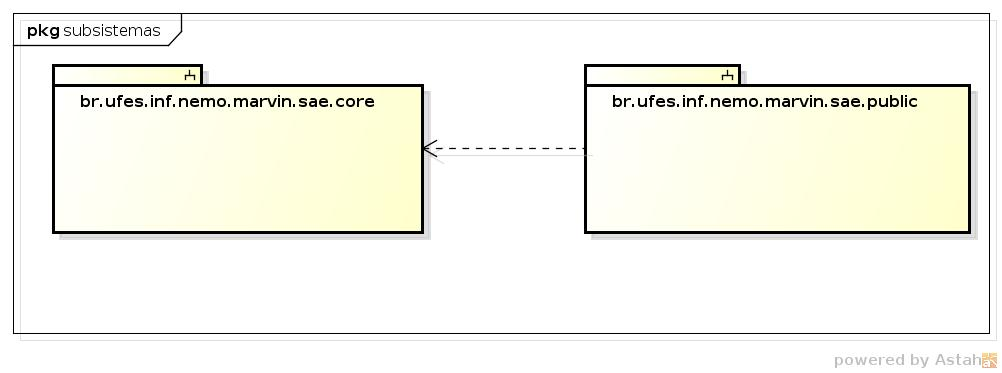
\includegraphics[width=0.8\textwidth]{figuras/projeto/fig-projeto-diagrama-pacotes}
	\caption{Pacotes que formam a arquitetura do SAE.}
	\label{fig-projeto-diagrama-pacotes}
\end{figure}



O módulo \texttt{br.ufes.inf.nemo.marvin.sae.core} contém as funcionalidades do subsistema \textbf{sae.core}, enquanto o módulo \texttt{br.ufes.inf.nemo.marvin.sae.public} contém as funcionalidades do subsistema \textbf{sae.public}. Mais à frente iremos detalhar um pouco mais as subdivisões desses módulos.


Os módulos principais do SAE são ainda subdivididos em camadas segundo a arquitetura que pode ser verificada na Figura~\ref{fig-projeto-arquitetura-sistema}. O sistema SAE foi divido em três camadas, sendo elas: apresentação (\textit{Presentation Tier}), negócio (\textit{Business Tier}) e acesso a dados (\textit{Data Access Tier}). Esta Figura mostra, também, as tecnologias Java associadas a cada pacote. Tais tecnologias foram abordadas na Seção~\ref{sec-referencial-desenvolvimento-web}.

\begin{figure}[h]
	\centering
	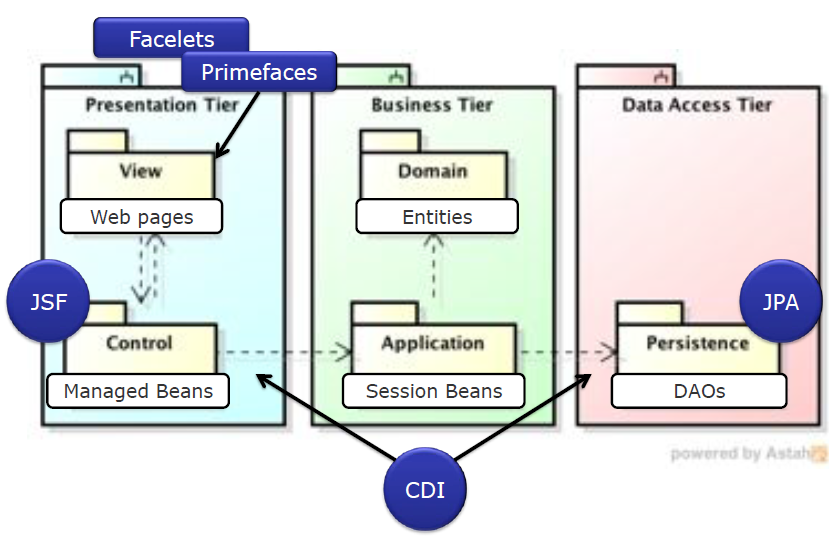
\includegraphics[width=0.8\textwidth]{figuras/projeto/fig-projeto-arquitetura-sistema}
	\caption{SAE - Arquitetura - Sistema~\cite{lima-pg15}.}	
	\label{fig-projeto-arquitetura-sistema}
\end{figure}

A Figura~\ref{fig-projeto-arquitetura-pacotes} exibe os pacotes do sistema SAE. Como podemos perceber, os pacotes foram agrupados pelos módulos principais e pelas camadas da arquitetura. A seguir iremos detalhar um pouco mais cada um deles.

\begin{figure}[h]
	\centering
	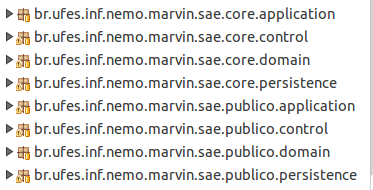
\includegraphics[width=0.45\textwidth]{figuras/projeto/fig-projeto-arquitetura-pacotes}
	\caption{SAE - Implementação - Pacotes.}
	\label{fig-projeto-arquitetura-pacotes}
\end{figure}




\subsection{Camada de Apresentação}
\label{sec-projeto-arquitetura-sistema-camada-apresentacao}

A \textbf{camada de apresentação} foi subdividida em visão (\textit{View}) e controle (\textit{Control}). A parte da visão é formada pelas páginas Web. A parte de controle contém os controladores que realizam a comunicação entre a interface e a aplicação.



A estrutura Web do sistema SAE, cujas páginas Web fazem parte da visão da camada de apresentação está organizada conforme a Figura~\ref{fig-projeto-arquitetura-paginas-web}. Existe uma pasta raiz chamada \texttt{WebContent} que contém todos os arquivos da visão. Ela possui duas subpastas que representam os módulos do SAE: \texttt{sae/core} e \texttt{sae/public}. Dentro de cada uma dessas, uma nova pasta foi criada para tratar cada caso de uso de forma separada. Isso ajuda na organização e caso seja necessário criar um novo caso de uso, basta adicionar uma nova pasta e os arquivos necessários. A subpasta \texttt{sae/public} ainda foi divida em \texttt{search}, para os casos de uso de consulta e \texttt{alumni} para os casos de usos relacionado aos egressos. 

\begin{figure}[h]
	\centering
	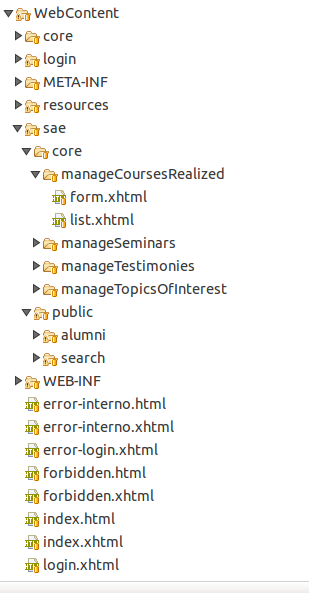
\includegraphics[width=0.35\textwidth]{figuras/projeto/fig-projeto-arquitetura-paginas-web}
	\caption{SAE - Implementação - Páginas Web}
	\label{fig-projeto-arquitetura-paginas-web}
\end{figure}

As pastas que implementam os casos de uso seguem um padrão que foi definido no framework do \textit{nemo-utils} (cf.\ Seção~\ref{sec-projeto-framework-nemo-utils}). Esse padrão de visão consiste em duas páginas, sendo a primeira chamada \texttt{form.xhtml}, que é responsável por elencar os dados das entidades para que possam ser modificados e armazenados no banco de dados. Já a página \texttt{list.xhtml} é responsável por recuperar e exibir para o usuário as informações da entidade que estão armazenadas no banco de dados.


Dentro da pasta raiz \texttt{WebContent}, temos as páginas \texttt{index.html} e \texttt{index.xhtml} que são as páginas iniciais do sistema. As páginas \texttt{error-interno.xhtml} e \texttt{error-interno.html} que serão utilizas para tratar de erros internos do servidor. As páginas \texttt{forbidden.html} e \texttt{forbidden.xhtml} que são usadas para o caso do usuário tentar acessar uma página que não tenha acesso. Temos ainda as páginas \texttt{login.xhtml} e \texttt{error-login.xhtml} que são as páginas do formulário de login e de erro ao efetuar o login respectivamente.



O decorador será utilizado para definir o layout da página e o menu que está sendo utilizado. A pasta \texttt{resources} contém a subpasta \texttt{default} que contém o decorador. 



\subsection{Camada de Negócio}
\label{sec-projeto-arquitetura-sistema-camada-negócio}

A \textbf{camada de negócio} foi subdividida em domínio (\textit{Domain}) e aplicação (\textit{Application}). A parte do domínio é formada pelas entidades do negócio, enquanto a aplicação contém as validações dos dados e implementação dos casos de uso (funcionalidades do sistema).

Os pacotes \texttt{sae.core.domain} e \texttt{sae.public.domain} contêm a definição das entidades do sistema SAE. Cada uma dessas entidades está definida em um arquivo \texttt{*.java} e já realiza o mapeamento objeto-relacional para o banco de dados. Através desse mapeamento, o JPA irá criar os objetos no banco de dados automaticamente, sem precisar de nenhuma intervenção do desenvolvedor. É nesse momento que é realizado também o relacionamento entre as classes do sistema utilizando as anotações \texttt{@OneToMany}, \texttt{@ManyToOne} ou \texttt{@ManyToMany} de JPA. Por fim, nesse pacote existe um arquivo para cada classe com o mesmo nome e um ``\_'' no final (chamada de \textit{static meta-model} ou metamodelo estático), que declara os atributos que poderão ser utilizados para realizar as consultas no banco de dados utilizando os conceitos de Criteria API. Essas consultas serão implementadas na camada de persistência.

Os pacotes \texttt{sae.core.application} e \texttt{sae.public.application} contêm os componentes que fazem a comunicação entre a apresentação (controladores) e a persistência (DAOs), implementando as funcionalidades do sistema descritas em seus casos de uso (cf.\ Cap.~\ref{sec-requisitos}). Faz também as validações das informações antes de chamar os métodos de acesso a dados. Essas validações serão feitas ao tentar criar ou modificar uma entidade.





\subsection{Camada de Acesso a Dados}
\label{sec-projeto-arquitetura-sistema-camada-acesso-dados}

A \textbf{camada de acesso a dados} possui uma única parte responsável pela persistência (\textit{Persistence}) representada pelos pacotes \texttt{sae.core.persistence} e \texttt{sae.public.per\-sistence}, que contêm os objetos responsáveis por fazer a comunicação com o banco de dados. Esses objetos são conhecidos como DAO (cf.\ Seção~\ref{sec-referencial-desenvolvimento-web-JPA}) e serão responsáveis por armazenar e recuperar os dados do banco de dados.

Sobre a arquitetura do banco de dados, conforme explicado anteriormente, o sistema SAE utiliza o JPA para fazer o mapeamento objeto relacional e, através desse mapeamento, o próprio JPA irá criar os objetos no banco de dados automaticamente. Com isso, foi utilizada a anotação \texttt{@Entity} nas classes do domínio para realizar a persistência dos dados.









% ========================================================================================
%   Framework nemo-utils
% ========================================================================================
\section{Framework \textit{nemo-utils}}
\label{sec-projeto-framework-nemo-utils}

Nesta seção vamos falar um pouco sobre o framework \textit{nemo-utils} \footnote{nemo-utils -- https://github.com/nemo-ufes/nemo-utils}, que foi utilizado para implementar o sistema SAE. No Documento de Requisitos, a \textbf{RNF07} diz que ``\textit{O desenvolvimento do sistema deve explorar o potencial de reutilização de componentes, tanto no que se refere ao desenvolvimento com reúso quanto ao desenvolvimento para reúso}''. Assim, foi utilizado o framework \textit{nemo-utils} que provê uma série de facilidades, pois ele já implementa as operações básicas entre a aplicação e o banco de dados de uma forma genérica, bastando ao desenvolver adaptar os códigos para as entidades do domínio do seu problema. Com isso, não foi necessário despender tempo criando funcionalidades que já estavam implementadas no framework. 

A maioria dos arquivos dos pacotes \texttt{sae.core.control} e \texttt{sae.public.control}  herdam da classe \texttt{CrudController} do \textit{nemo-utils}. Essa classe é responsável por armazenar temporariamente os dados das páginas Web e depois fazer a comunicação com a camada de aplicação. Em algumas páginas, também são responsáveis por carregar os dados dos componentes \texttt{selectOneMenu} do \textbf{PrimeFaces}. Além disso, realizam os filtros de pesquisa através do método \texttt{initFilters}.


A maioria dos arquivos dos pacotes \texttt{sae.core.application} e \texttt{sae.public.appli\-cation} herdam da classe \texttt{CrudServiceBean} do \textit{nemo-utils}. Essa classe é responsável por realizar as validações e por fazer a comunicação com a camada de acesso a dados. Essa classe possui alguns métodos responsáveis pelas validações. Estes métodos são vazios na classe \texttt{CrudServiceBean} e precisam ser implementados de acordo com as validações a serem realizadas em cada caso, são eles:

\begin{itemize}	
	\item \texttt{validateCreate --} responsável por fazer as validações ao tentar criar uma nova entidade no sistema. Também possui validações para evitar que dados duplicados sejam inseridos no sistema;
	
	\item \texttt{validateUpdate --} responsável por fazer as validações ao tentar atualizar os dados de uma entidade já existente no sistema. Também possui validações para evitar que dados duplicados sejam inseridos no sistema;
	
	\item \texttt{validateDelete --} responsável por fazer as validações ao tentar excluir os dados de uma entidade já existente no sistema. Em alguns casos, algumas classes não podem ser excluídas se tiverem algum relacionamento com outra classe no sistema. Por exemplo, não é possível excluir um professor que possua uma turma.
\end{itemize}


Utilizando o conceito de herança da programação orientada a objetos, quase todas as entidades do domínio herdam da classe \texttt{PersistentObjectSupport}, que é uma implementação padrão para objetos persistentes que utiliza EJB 3 como padrão de anotações para persistência. Essas classes estão nos pacotes \texttt{sae.core.domain} e \texttt{sae.public.domain} e possuem os seguintes atributos: \texttt{serialVersionUID, uuid, id e version}. Nesse caso, é importante saber que o campo \texttt{id} será usado para identificar unicamente uma entidade no banco de dados, o campo \texttt{uuid} é um número gerado aleatoriamente para diferenciar unicamente uma entidade e o campo \texttt{version} identifica a versão da entidade.



Por último, os arquivos dos pacotes \texttt{sae.core.persistence} e \texttt{sae.public.per\-sistence} herdam da classe \texttt{BaseJPADAO} do \textit{nemo-utils}. Essa classe é responsável por realizar as operações no banco de dados, sendo elas: consulta, modificação, inserção e exclusão de dados. Todas as consultas são realizadas utilizando os conceitos de Criteria API do JPA. Como as consultas que foram implementadas são bem simples utilizando poucas restrições, grande parte do código foi reaproveitado para todas as classes, alterando apenas o tipo e os atributos.










% ========================================================================================
%   Modelos FrameWeb
% ========================================================================================
\section{Modelos FrameWeb}
\label{sec-projeto-modelos-frame-web}

Nesta seção, serão exibidos os modelos FrameWeb que já foram citados anteriormente na Seção~\ref{sec-referencial-frameweb}. Esses modelos também estão divididos nas camadas da arquitetura do sistema, conforme citado na Seção~\ref{sec-projeto-arquitetura-sistema}.




\subsection{Modelo de Domínio}

%Apresentamos primeiramente o \textbf{Modelo de Domínio}. 
Os mapeamentos de persistência são meta-dados das classes de domínio que permitem que os \textit{frameworks} ORM transformem objetos que estão na memória em linhas de tabelas no banco de dados relacional. Por meio de mecanismos leves de extensão da UML, como estereótipos e restrições, adicionamos tais mapeamentos ao diagrama de classes de domínio. Apesar de tais configurações serem relacionadas mais à persistência do que ao domínio, elas são representadas no Modelo de Domínio porque as classes que são mapeadas e seus atributos são exibidas neste diagrama. A Figura~\ref{fig-projeto-core-modelo-dominio} mostra o modelo de domínio para o módulo \texttt{sae.core}.

\begin{figure}[!h]
	\centering
	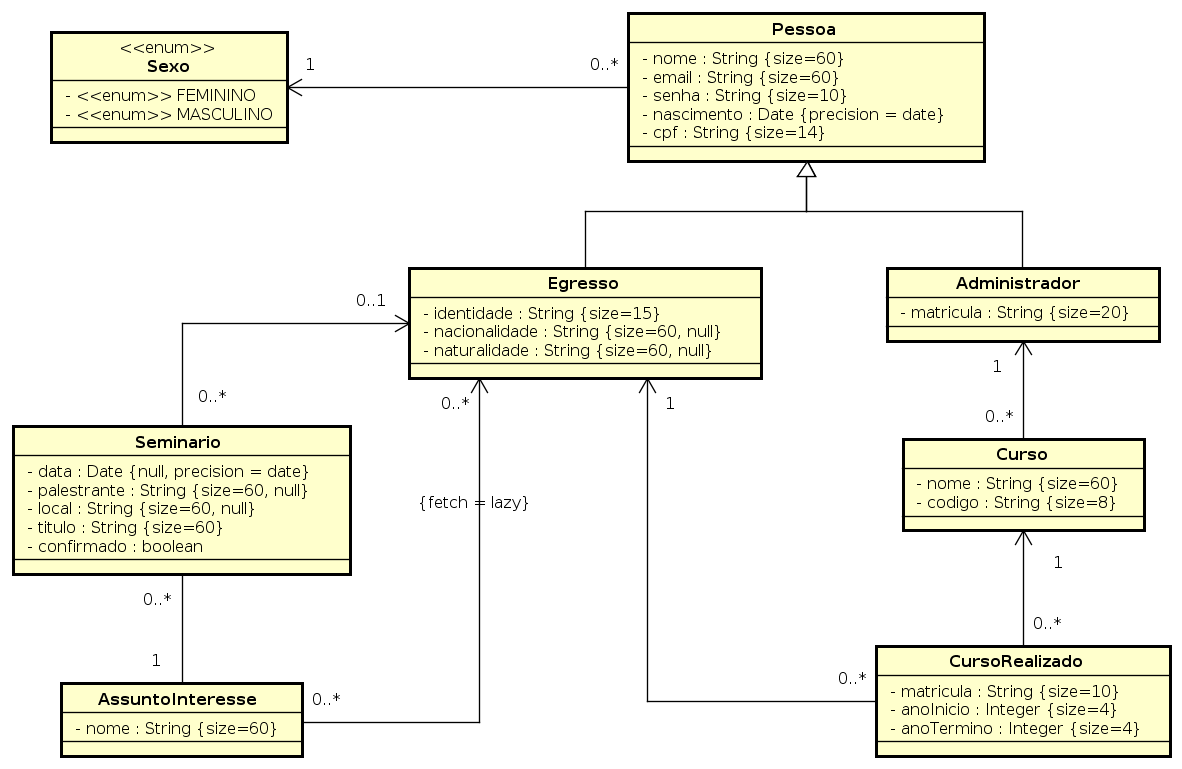
\includegraphics[width=0.88\textwidth]{figuras/projeto/fig-projeto-core-modelo-dominio}
	\caption{FrameWeb - sae.core - Modelo Domínio.}
	\label{fig-projeto-core-modelo-dominio}
\end{figure}



Podemos observar nesta figura que quase todos atributos tem tamanho (\texttt{size}) definido. As classe \textbf{Egresso} e \textbf{Seminário} têm atributos do tipo data, na restrição destes atributos informamos se precisão vai ser \textit{time}, armazenando no banco de dados somente a hora, \textit{date}, apenas a data, ou \textit{timestamp} armazenado ambos, data e hora. Neste último caso não é preciso colocar na restrição pois é a opção \textit{default}.

A associação entre as classes \textbf{Egresso} e \textbf{AssuntoInteresse} tem uma restrição \texttt{fetch} que indica qual a estratégia de recuperação do banco de dados. Nesta associação está especificada a opção \textit{lazy}, que significa que a recuperação vai ser no modo preguiçoso, ou seja, somente vai trazer do banco de dados quando precisar da informação.

A Figura~\ref{fig-projeto-public-modelo-dominio} mostra o modelo de domínio para o módulo \texttt{sae.public}. As classes \textbf{Sugestão} e \textbf{Depoimento} possuem atributos marcados com estereótipo \textit{lob}, isso significa que no banco de dados será criado um campo de tamanho grande como \textit{clob} que pode ter até 4GB de dados para armazenamento de texto e \textit{blob} que também pode ter até 4GB de dados binários, este último para armazenar informações digitais como imagens, áudios e vídeos.  

\begin{figure}[!h]
	\centering
	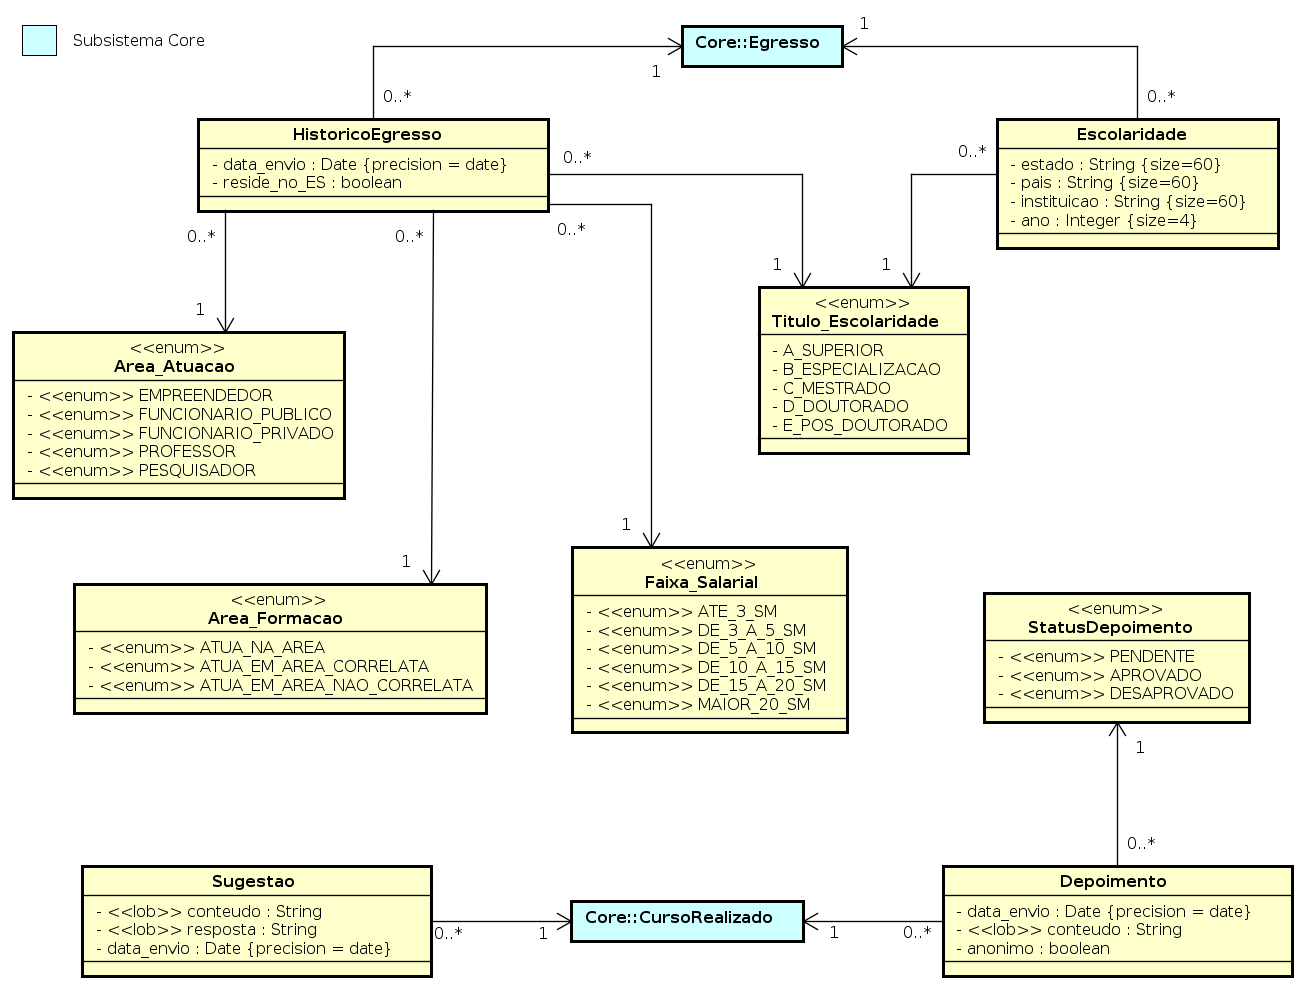
\includegraphics[width=0.8\textwidth]{figuras/projeto/fig-projeto-public-modelo-dominio}
	\caption{FrameWeb - Public - Modelo Domínio.}
	\label{fig-projeto-public-modelo-dominio}
\end{figure}

Todas as classes de domínio estendem de \textit{PersistentObjectSupport} do framework \textit{nemo-utils}, sendo que essa herança não é mostrada no diagrama com o intuito de não poluí-lo com várias associações.

Diferente da abordagem original do FrameWeb original proposto em 2007, todos os atributos que são não nulos tiveram a \textit{tag {not null}} omitida e os que são nulos tiveram a \textit{tag {null}} acrescida de forma a diminuir a poluição visual com repetições desnecessárias no diagrama.





\newpage
\subsection{Modelo de Navegação}

O \textbf{Modelo de Navegação} é um diagrama de classe da UML que representa os diferentes componentes que formam a camada de Apresentação, como páginas Web, formulários HTML e classes de ação. Esse modelo é utilizado pelos desenvolvedores para guiar a codificação das classes e componentes dos pacotes \textbf{Visão} e \textbf{Controle}.


Em formulários HTML, atributos representam campos do formulário, que devem ter seus tipos definidos de acordo com a biblioteca de componentes utilizada, como neste trabalho foi utilizado PrimeFaces os tipos ficarão com o prefixo ``p'' (ex.: \texttt{p.input}, \texttt{p.checkbox}, \texttt{p.button}, etc.). A classe de ação é o principal componente do modelo. Suas associações de dependência ditam o controle de fluxo quando uma ação é executada.



As funcionalidades criar, editar, excluir e visualizar (abreviadas de CRUD, do inglês \textit{create, read, update e delete}), seguem um mesmo fluxo de execução e de interação com o usuário. Tais funcionalidades são similares para todos os casos de uso cadastrais devido a utilização da ferramenta \textit{nemo-utils}. Esse fluxo de execução similar é representado pela Figura~\ref{fig-projeto-nemo-utils-modelo-navegacao} que é um modelo de apresentação genérico.

\begin{figure}[h]
	\centering
	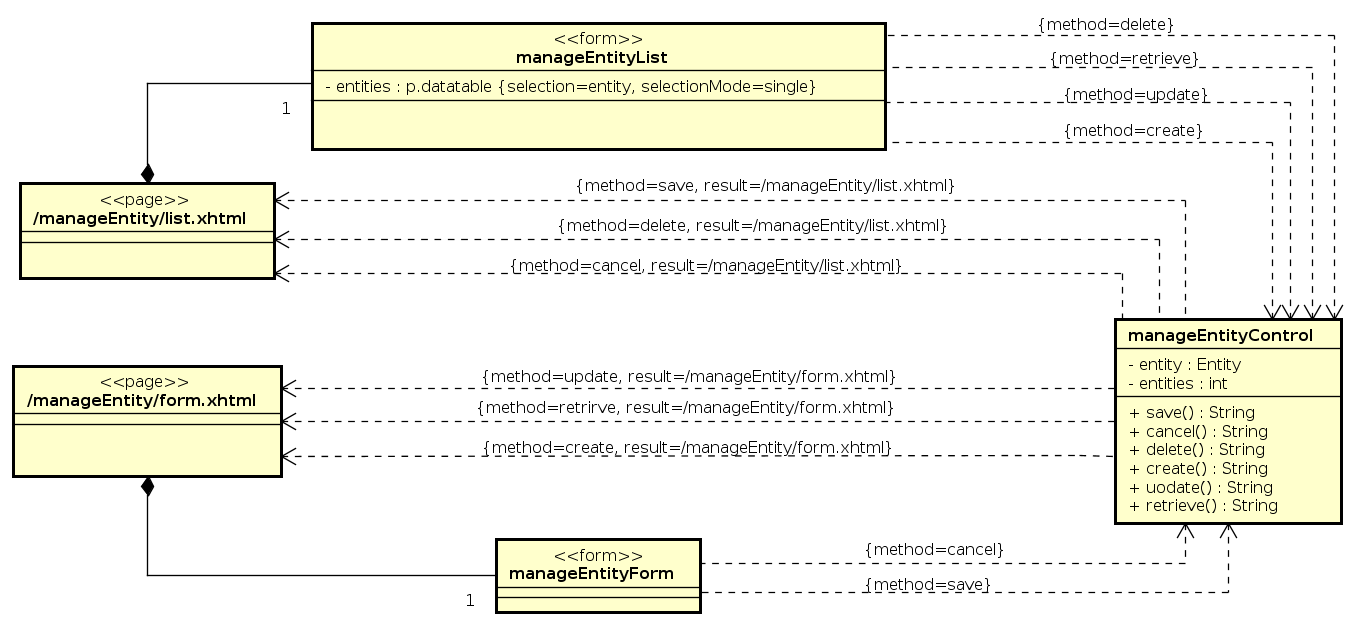
\includegraphics[width=0.9\textwidth]{figuras/projeto/fig-projeto-nemo-utils-modelo-navegacao}
	\caption{FrameWeb - \textit{nemo-utils} - Modelo Navegação~\cite{lima-pg15}.}
	\label{fig-projeto-nemo-utils-modelo-navegacao}
\end{figure}




Para os casos de uso que apresentam funções diferentes das CRUDs, o modelo anterior não pode ser aplicado. A Figura~\ref{fig-projeto-modelo-navegacao-consultarDepoimento} é um modelo de navegação para o caso de uso “Consultar Depoimento”. 

\begin{figure}[h]
	\centering
	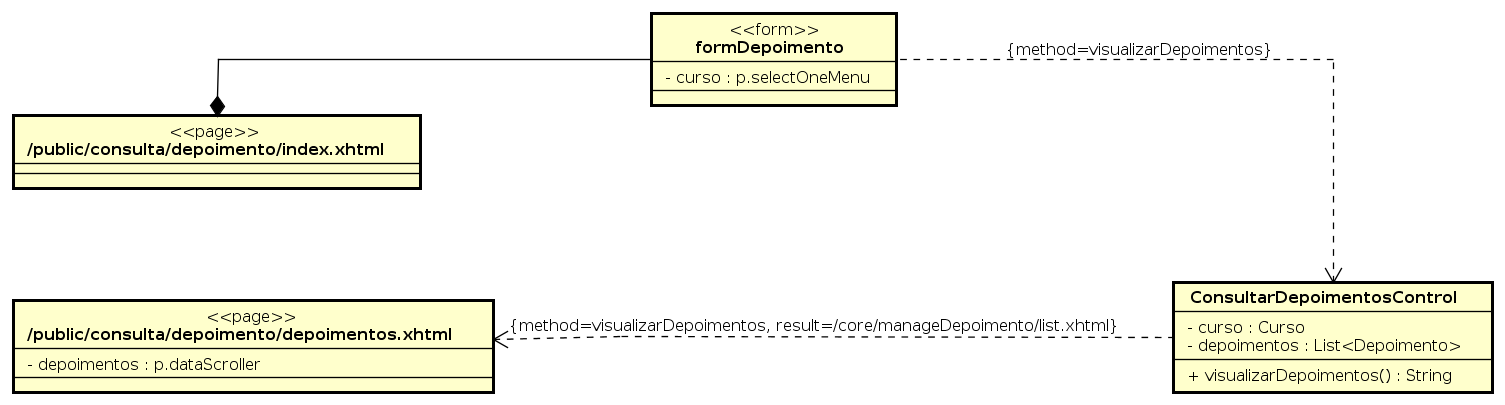
\includegraphics[width=0.9\textwidth]{figuras/projeto/fig-projeto-modelo-navegacao-consultarDepoimento}
	\caption{FrameWeb - Consultar Depoimentos - Modelo Navegação.}
	\label{fig-projeto-modelo-navegacao-consultarDepoimento}
\end{figure}


Podemos perceber que o modelo possui duas páginas web marcadas com estereótipo \texttt{<<page>>}, a pagina \textit{index.xhtml} possui um formulário marcado com estereótipo \texttt{<<form>>} que possui o atributo \textit{curso}, este é injetado via EL (Expression Language) na classe chamada \texttt{ConsultaControl} que representa o controlador. Após selecionado o curso, o formulário aciona o método \textit{visualizarDepoimento()} do controlador, o mesmo processa a requisição e mostra o resultado na página \textit{depoimentos.xhtml}.  






\subsection{Modelo de Aplicação}

O \textbf{Modelo de Aplicação} é um diagrama de classes da UML que representa as classes de serviço, responsáveis pela codificação dos casos de uso, e suas dependências. Esse diagrama é utilizado para guiar a implementação das classes do pacote \textbf{Aplicação} e a configuração das dependências entre os pacotes \textbf{Controle, Aplicação e Persistência}, ou seja, quais classes de ação dependem de quais classes de serviço e quais DAOs são necessários para que as classes de serviço alcancem seus objetivos~\cite{vitorFrameWeb}.


Todas as classes de aplicação que são cadastrais estendem de \textit{CrudServiceBean} do pacote \textit{nemo-utils}, porém com uma pequena alteração, foi adicionado a classe uma anotação \texttt{@PermitAll}, permitindo o controle de segurança. Tal classe está representada na Figura~\ref{fig-projeto-nemo-utils-modelo-aplicacao} de forma genérica (\texttt{Entity} é implementado como um politipo/tipo genérico \texttt{T} no código da classe). Da mesma forma dos diagramas anteriores essa herança não é mostrada no diagrama acima com o intuito de não poluir o diagrama com várias associações.


\begin{figure}[h]
	\centering
	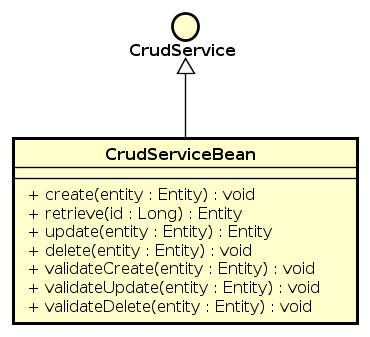
\includegraphics[width=0.3\textwidth]{figuras/projeto/fig-projeto-nemo-utils-modelo-aplicacao}
	\caption{FrameWeb - \textit{nemo-utils} - Modelo Aplicação~\cite{lima-pg15}.}
	\label{fig-projeto-nemo-utils-modelo-aplicacao}
\end{figure}



A Figura~\ref{fig-projeto-public-modelo-aplicacao} mostra o modelo de aplicação para o módulo \texttt{sae.public}. Já a Figura~\ref{fig-projeto-core-modelo-aplicacao} mostra o modelo de aplicação para o módulo \texttt{sae.core} .


\begin{figure}[h]
	\centering
	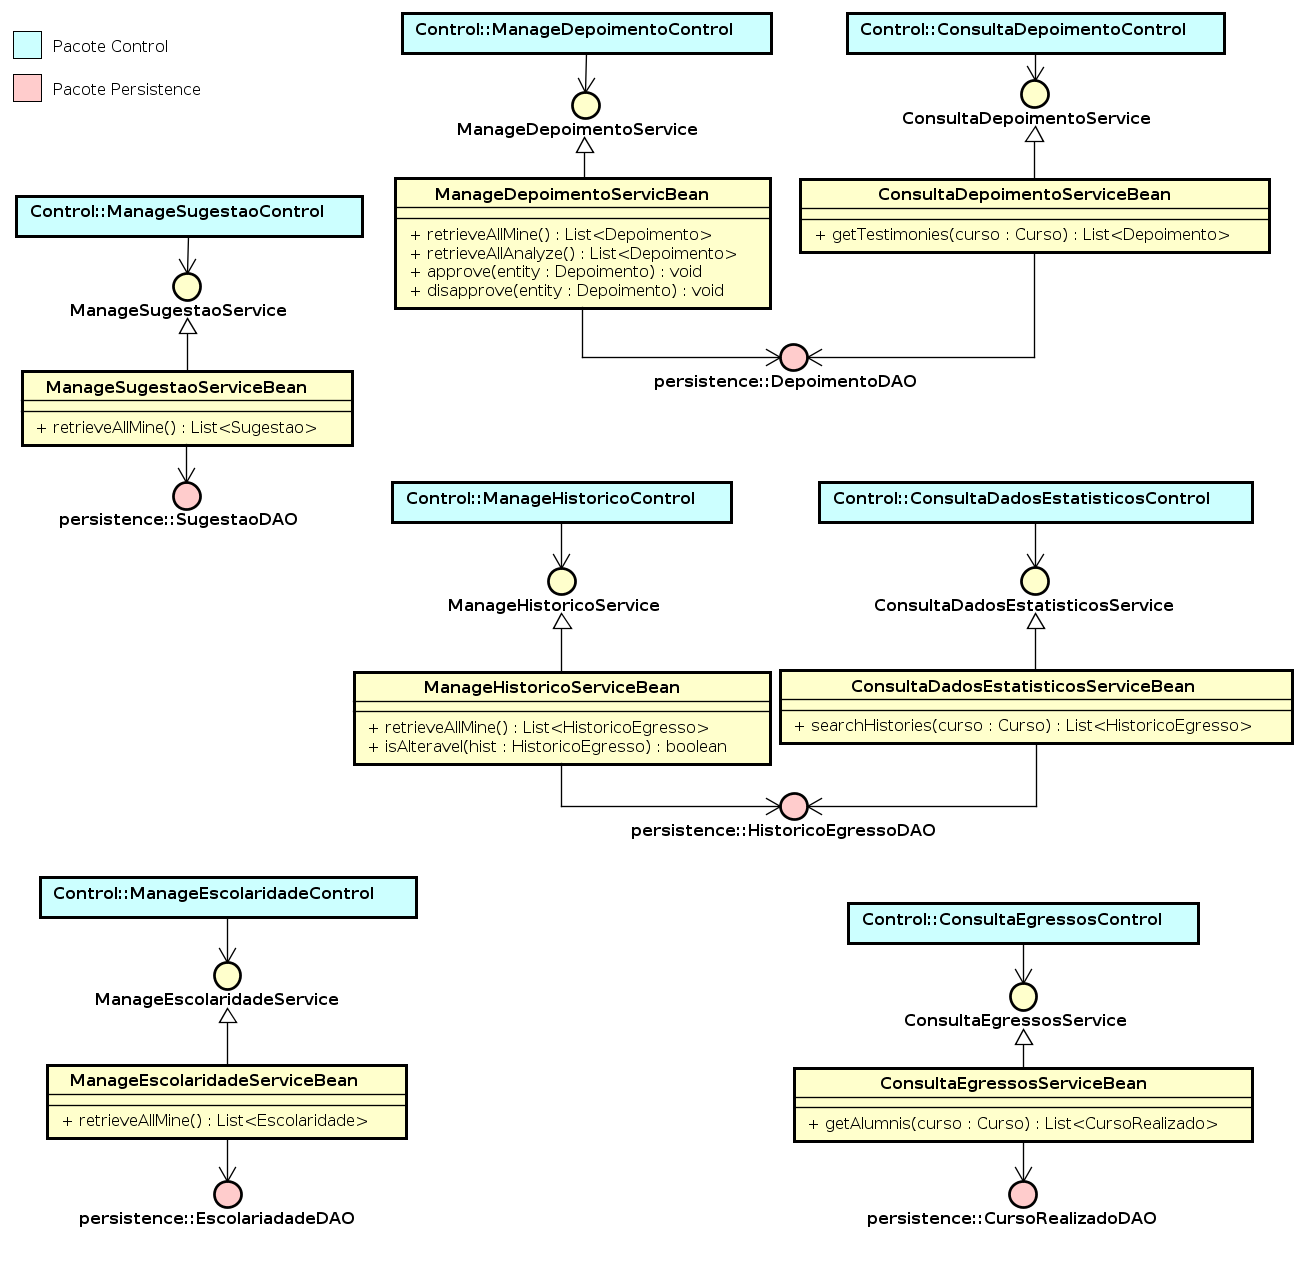
\includegraphics[width=0.9\textwidth]{figuras/projeto/fig-projeto-public-modelo-aplicacao}
	\caption{FrameWeb - Public - Modelo Aplicação.}
	\label{fig-projeto-public-modelo-aplicacao}
\end{figure}


\begin{figure}[h]
	\centering
	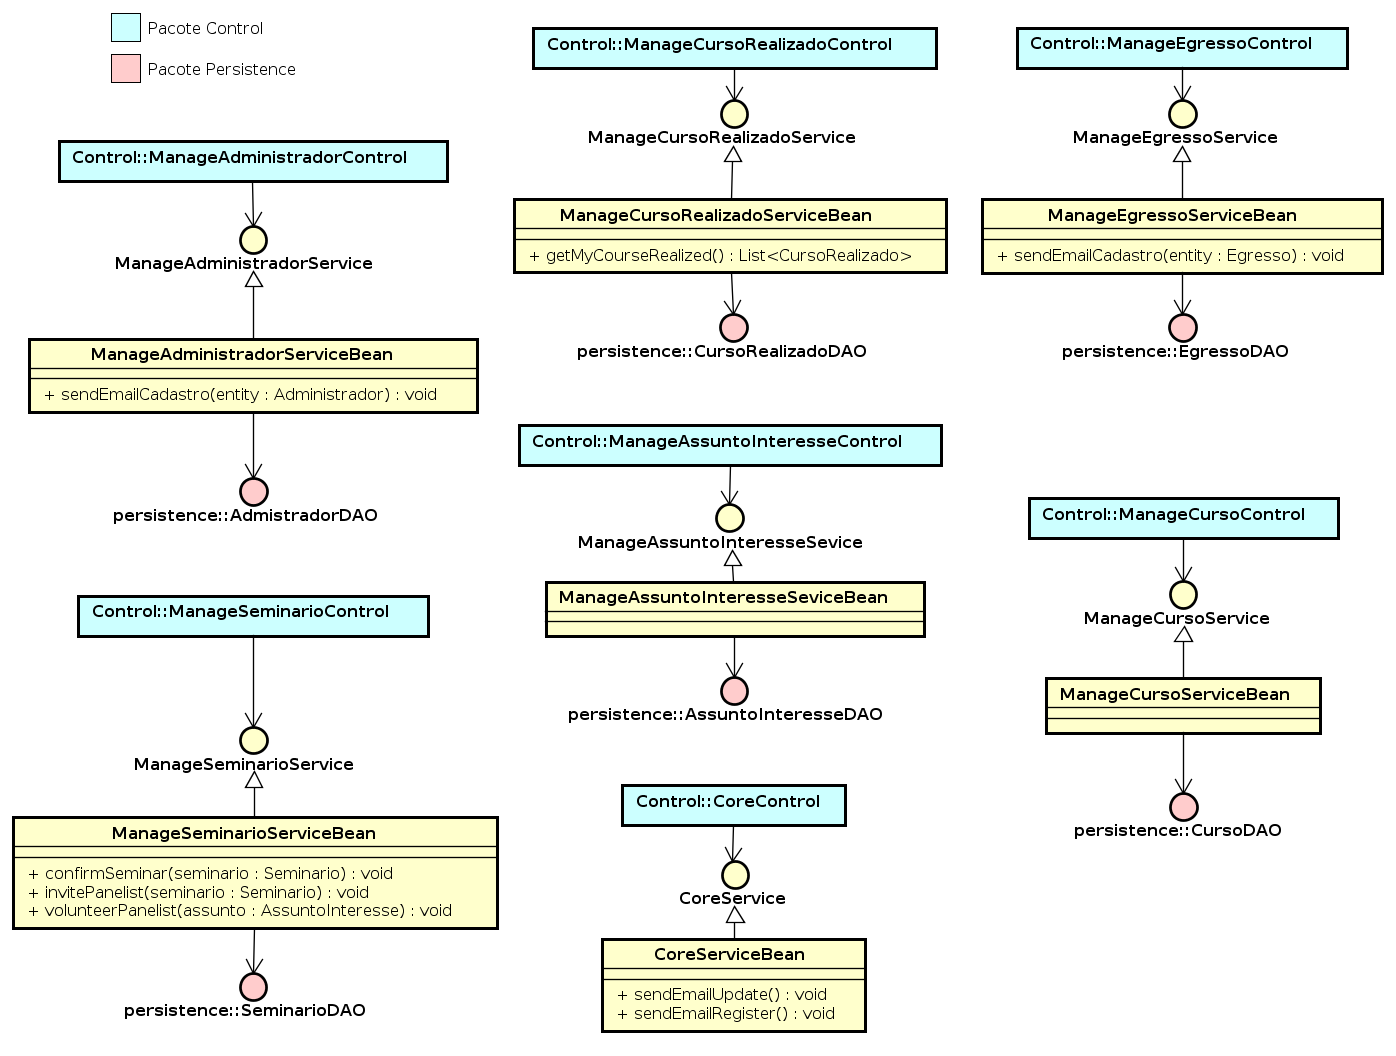
\includegraphics[width=1\textwidth]{figuras/projeto/fig-projeto-core-modelo-aplicacao}
	\caption{FrameWeb - Core - Modelo Aplicação.}
	\label{fig-projeto-core-modelo-aplicacao}
\end{figure}



\newpage
\subsection{Modelo de Persistência}

O FrameWeb indica a utilização do padrão de projeto DAO para a construção da camada de acesso a dados. O \textbf{Modelo de Persistência} é um diagrama de classes da UML que representa as classes DAO existentes, responsáveis pela persistência das instâncias das classes de domínio. Esse diagrama guia a construção das classes DAO, que pertencem ao pacote de persistência.


Para que não seja necessário repetir em cada interface DAO operações que são comuns a todas elas (ex.: \texttt{save(), delete(), retrieveById()}, etc.), podemos apresentar DAOs base que declaram esses métodos – novamente, uma interface e várias implementações. Automaticamente, todas as interfaces DAO de todos os diagramas herdam as definições da interface base, ocorrendo o mesmo com as implementações concretas de cada tecnologia de persistência, sem que isso precise estar explícito no diagrama. A Figura~\ref{fig-projeto-nemo-utils-modelo-persistencia} exibe as classes bases do \textit{nemo-utils}.

\begin{figure}[h]
	\centering
	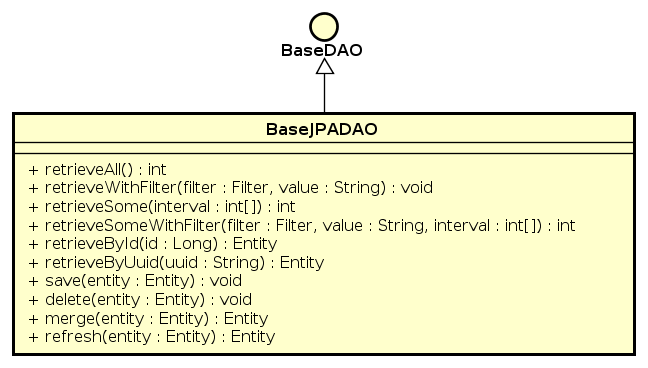
\includegraphics[width=0.6\textwidth]{figuras/projeto/fig-projeto-nemo-utils-modelo-persistencia}
	\caption{FrameWeb - \textit{nemo-utils} - Modelo Persistência~\cite{lima-pg15}.}
	\label{fig-projeto-nemo-utils-modelo-persistencia}
\end{figure}

Tanto a interface \textbf{BaseDAO} quanto a classe \textbf{BaseJPADAO} são declaradas usando tipos genéricos, deixando a cargo de suas subinterfaces e subclasses a especificação da classe gerenciada por cada DAO. O DAO base define métodos para recuperar todos os objetos de uma determinada classe, recuperar um objeto dado seu identificador, salvar e excluir um objeto. Também não será necessário exibir os métodos do DAO na implementação e na interface, basta modelá-los em apenas um dos dois. No caso do DAO Base, subentende-se que todos os métodos públicos de BaseJPADAO são definidos na interface BaseDAO.

Segundo os padrões estabelecidos por FrameWeb, todas as interfaces DAO são subinterfaces de BaseDAO, enquanto todas as implementações JPA são subclasses de BaseJPADAO, herdando todos os métodos básicos, por exemplo: \texttt{retrieveAll(), save(), delete(), retrieveById()}. Os demais métodos que foram declarados no diagrama se referem a consultas específicas que devem ser disponibilizadas para o funcionamento de determinados casos de uso. 

As Figuras~\ref{fig-projeto-public-modelo-persistencia} e~\ref{fig-projeto-core-modelo-persistencia} são os modelos de persistência para os módulos \texttt{sae.public}  e \texttt{sae.core}, respectivamente.

\begin{figure}[h]
	\centering
	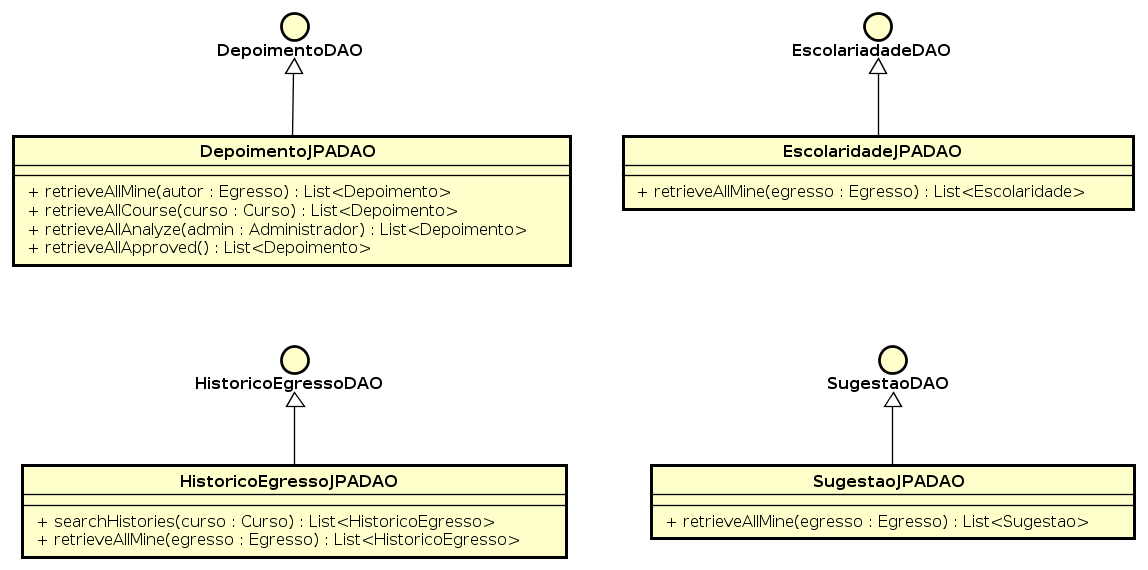
\includegraphics[width=0.9\textwidth]{figuras/projeto/fig-projeto-public-modelo-persistencia}
	\caption{FrameWeb - Public - Modelo Persistência.}
	\label{fig-projeto-public-modelo-persistencia}
\end{figure}


\begin{figure}[h]
	\centering
	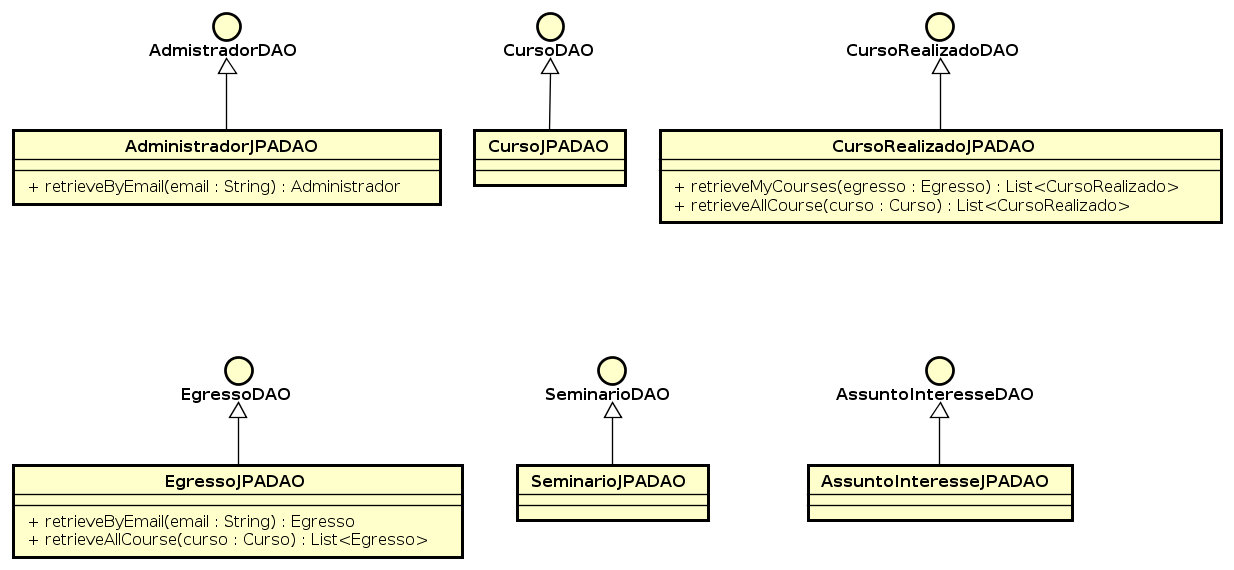
\includegraphics[width=0.9\textwidth]{figuras/projeto/fig-projeto-core-modelo-persistencia}
	\caption{FrameWeb - Core - Modelo Persistência.}
	\label{fig-projeto-core-modelo-persistencia}
\end{figure}



Como é possível perceber, o Modelo de Persistência não define nenhuma extensão da UML para representar os conceitos necessários da camada de acesso a dados, mas apenas regras que tornam essa modelagem mais simples e rápida, por meio da definição de padrões.
















% ========================================================================================
%  Apresentando o Sistema
% ========================================================================================
\section{Apresentação do Sistema}
\label{sec-projeto-apresentacao-sistema}

Nesta seção, apresentamos o sistema por meio de uma série de capturas de tela. A Figura~\ref{fig-projeto-apresentacao-login} mostra a tela inicial de login no sistema. 


\begin{figure}[h]
	\centering
	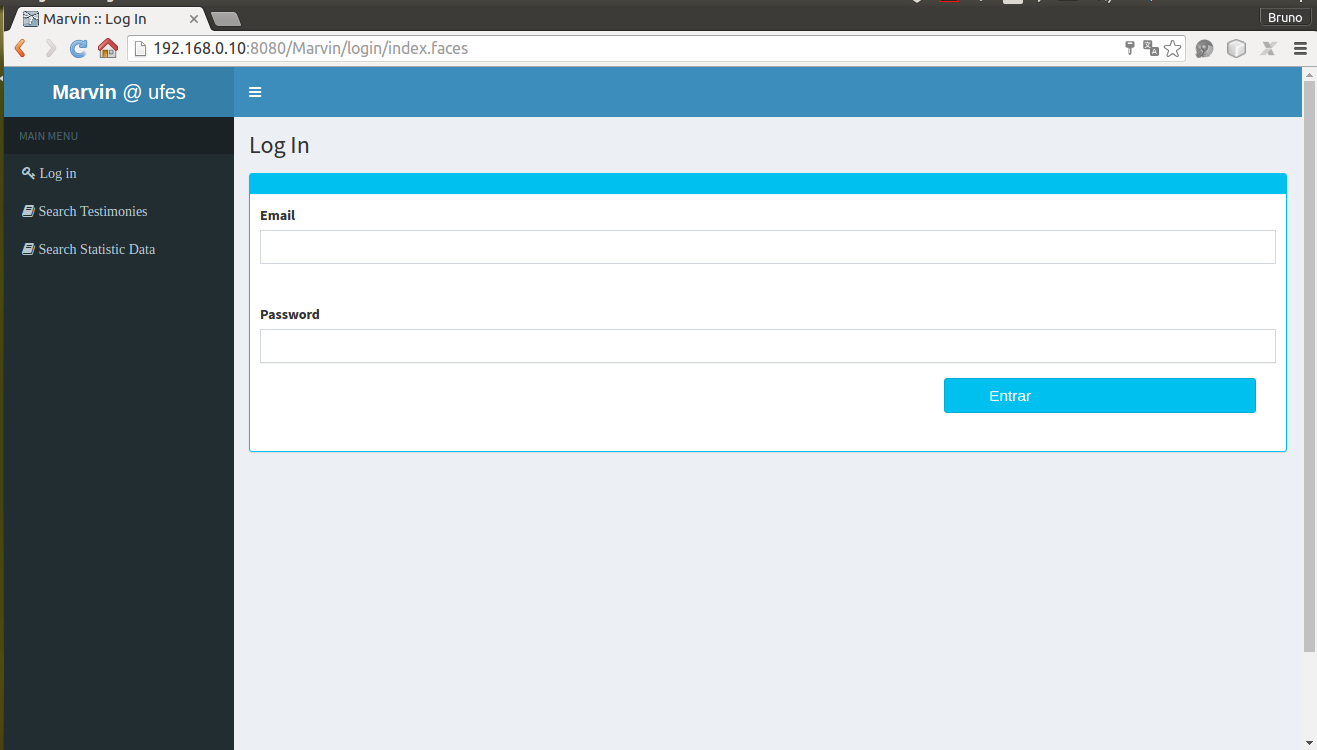
\includegraphics[width=0.75\textwidth]{figuras/projeto/fig-projeto-apresentacao-login}
	\caption{SAE - Tela Login.}
	\label{fig-projeto-apresentacao-login}
\end{figure}

Podemos ver no canto esquerdo da tela uma barra com os menus do sistema, quando um usuário faz login no sistema aparecerão nesta barra as funções que ele tem acesso. A parte á direita é destinada a exibir as informações do sistema.



No Documento de Requisitos, a \textbf{RNF-4} diz que ``O sistema deve controlar o acesso às funcionalidades''. Pensando nisso, o sistema SAE implementou login e senha para que os seus usuários realizem o acesso e também trata a questão da sessão expirada. A seguir iremos explicar essas questões.

O login utilizará e-mail e senha. O campo do e-mail possui validação para verificar se o mesmo é válido. O campo da senha aceita qualquer caractere alfanumérico e possui tamanho máximo 15. Caso o e-mail e senha informados não correspondam a nenhum usuário, será redirecionado para uma página de erro de login, conforme a Figura~\ref{fig-projeto-apresentacao-login-erro}.

\begin{figure}[h]
	\centering
	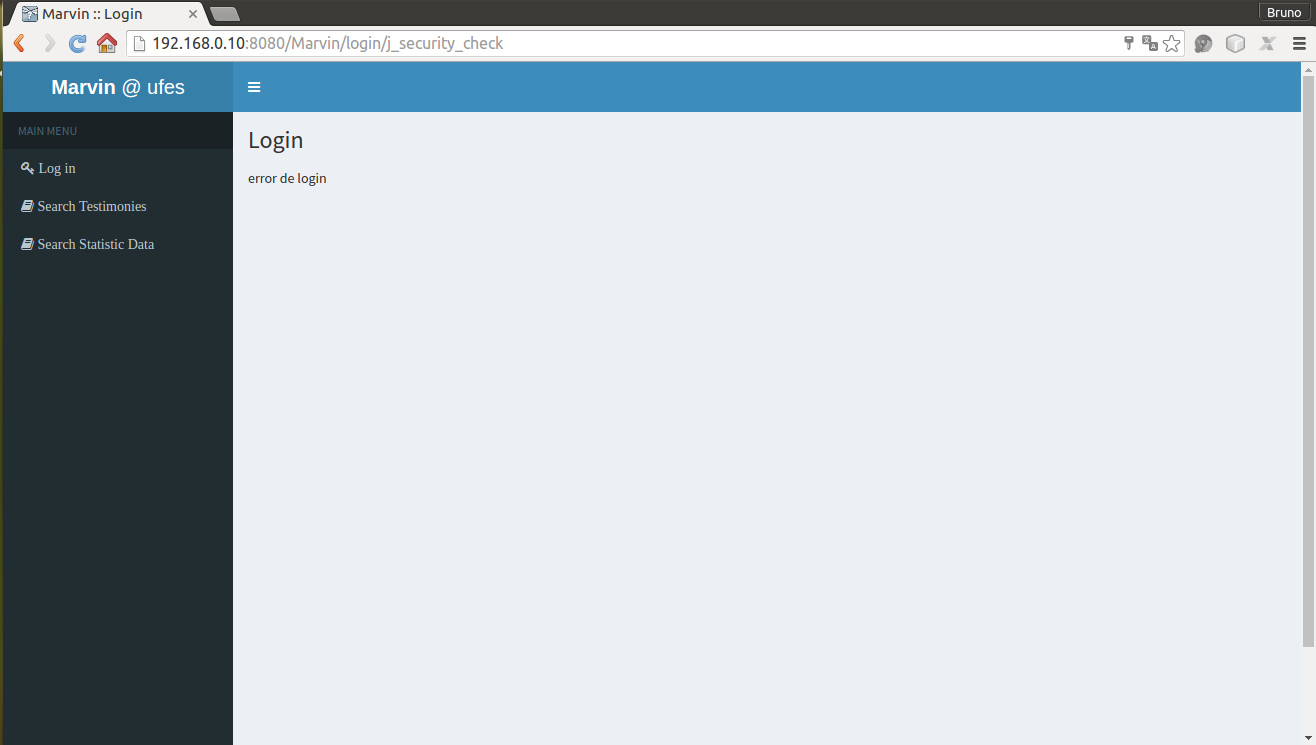
\includegraphics[width=0.75\textwidth]{figuras/projeto/fig-projeto-apresentacao-login-erro}
	\caption{SAE - Erro Login.}
	\label{fig-projeto-apresentacao-login-erro}
\end{figure}



Os menus do sistema irão variar de acordo com o usuário. A Figura~\ref{fig-projeto-tela-inicial-egresso} exibe a tela inicial do Egresso no menu à esquerda aparece apenas as funcionalidades que o egresso tem acesso.

\begin{figure}[h]
	\centering
	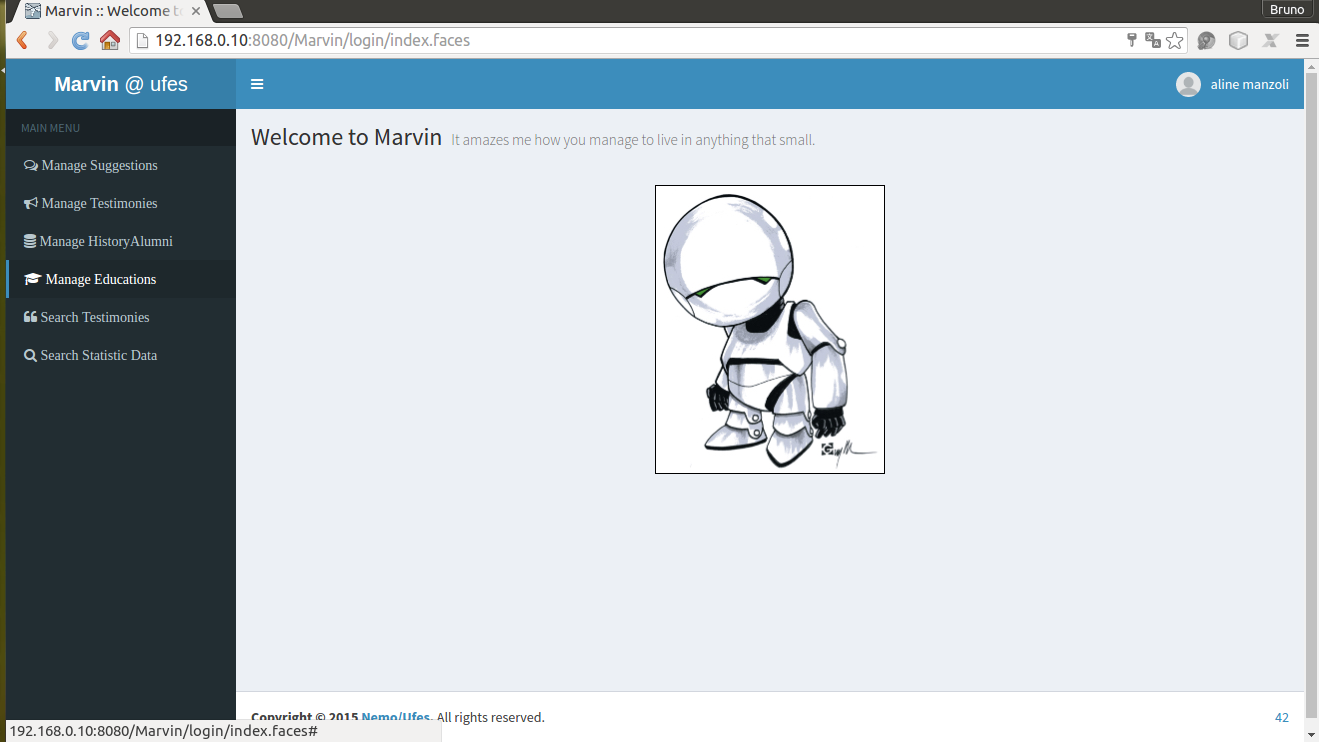
\includegraphics[width=0.75\textwidth]{figuras/projeto/fig-projeto-apresentacao-tela-inicial-egresso}
	\caption{SAE - Tela inicial Egresso.}
	\label{fig-projeto-tela-inicial-egresso}
\end{figure}


A Figura~\ref{fig-projeto-apresentacao-tela-reponsiva-administrador} exibe a tela inicial do administrador após realizar o login em um \textit{smartphone}. Como o Marvin utiliza um layout responsivo, haverá diferenças com a visualização em computador. Podemos notar na figura mais à esquerda que a parte de menus ficar oculta e, para visualizar o menu, como mostra a figura mais à direita, é preciso clicar no ícone ao lado do nome de usuário.


\begin{figure}[h]
	\centering
	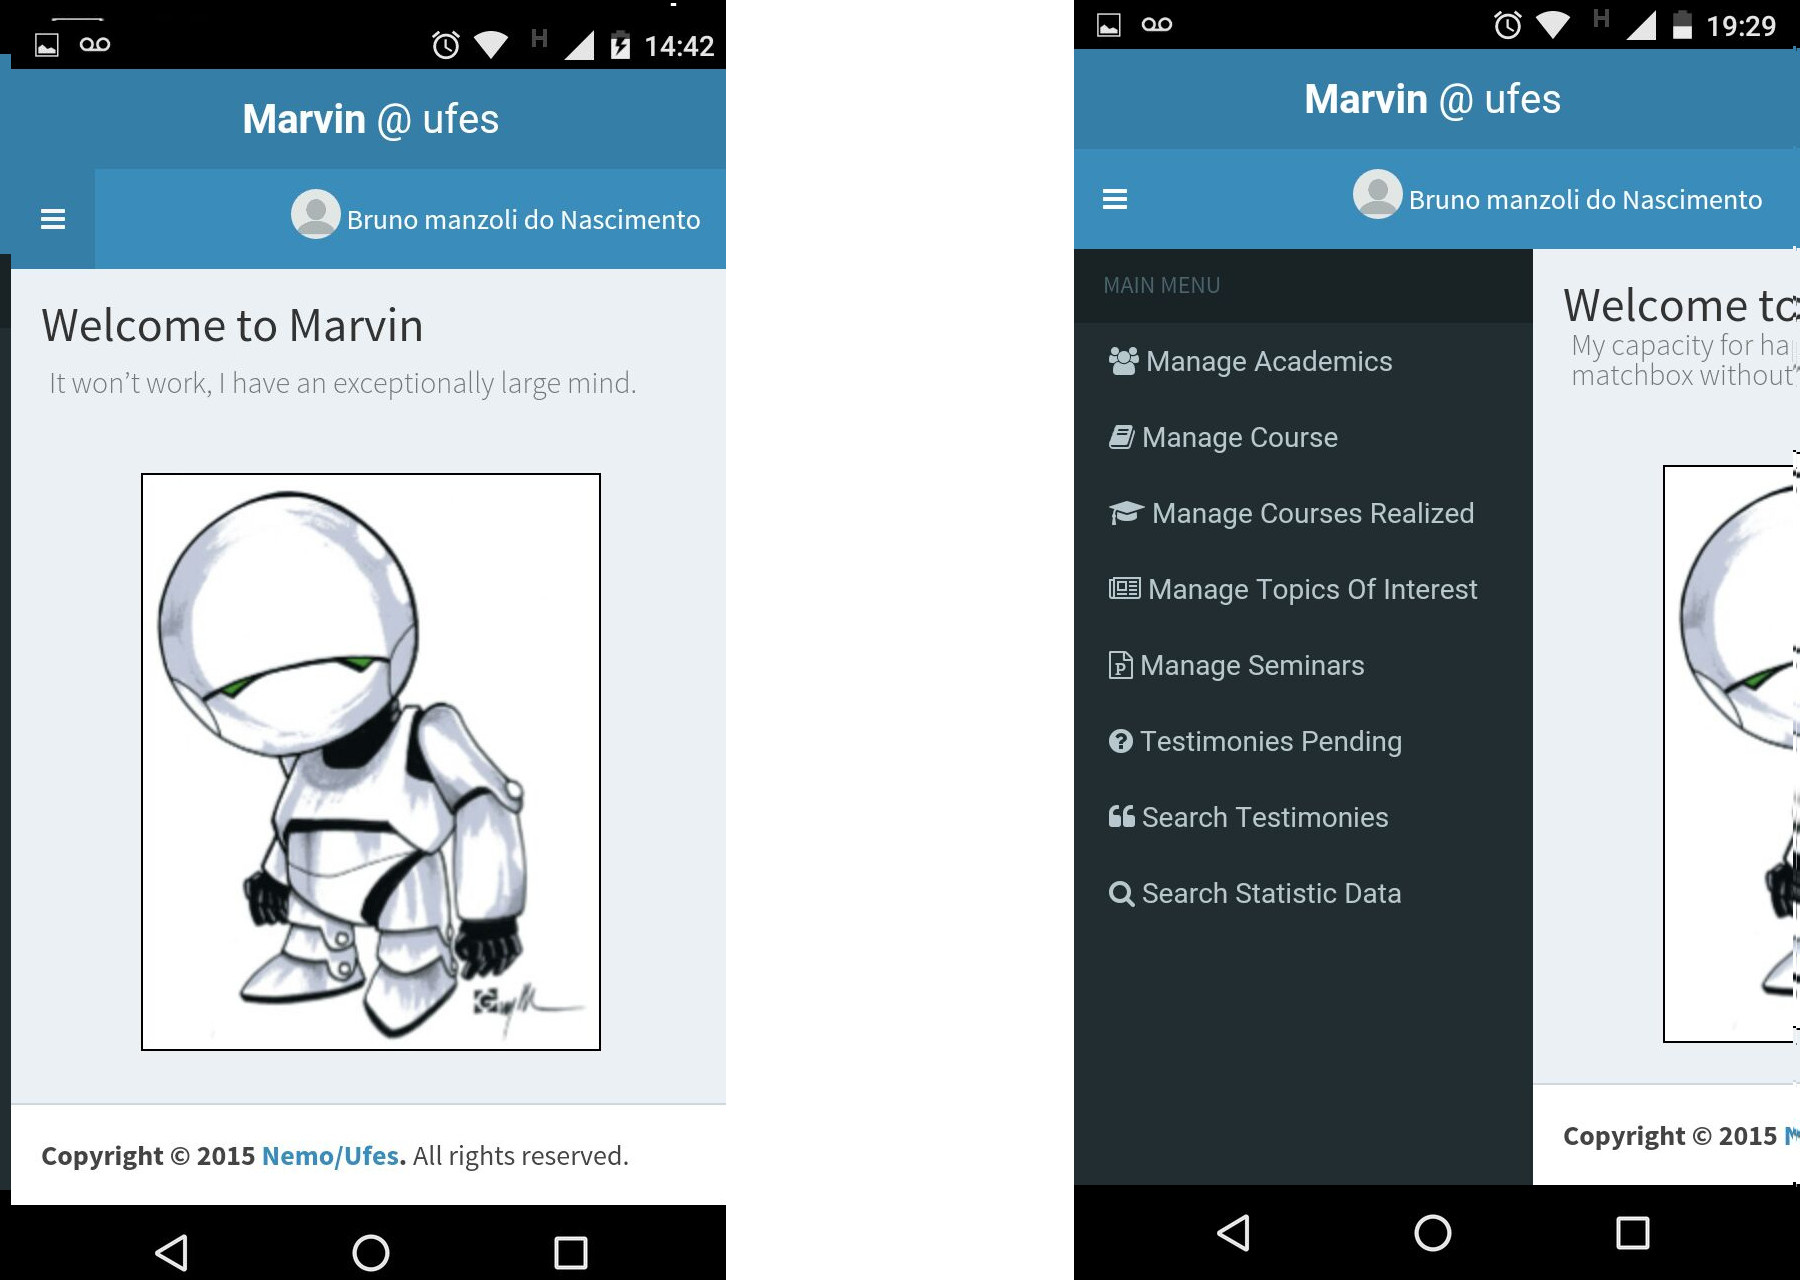
\includegraphics[width=0.7\textwidth]{figuras/projeto/fig-projeto-apresentacao-tela-reponsiva-administrador}
	\caption{SAE - Tela Mobile de Administrador.}
	\label{fig-projeto-apresentacao-tela-reponsiva-administrador}
\end{figure}


As funcionalidades que são relacionadas a cadastro, onde se pode criar um novo item, visualizar um item, alterar um item existente ou excluir um item, têm telas que seguem um padrão sendo uma para listar os itens cadastrados e outra para visualizar ou alterar os dados de um item. A Figura~\ref{fig-projeto-apresentacao-course-list} exibe a tela que lista os cursos cadastrados no sistema.

\begin{figure}[h]
	\centering
	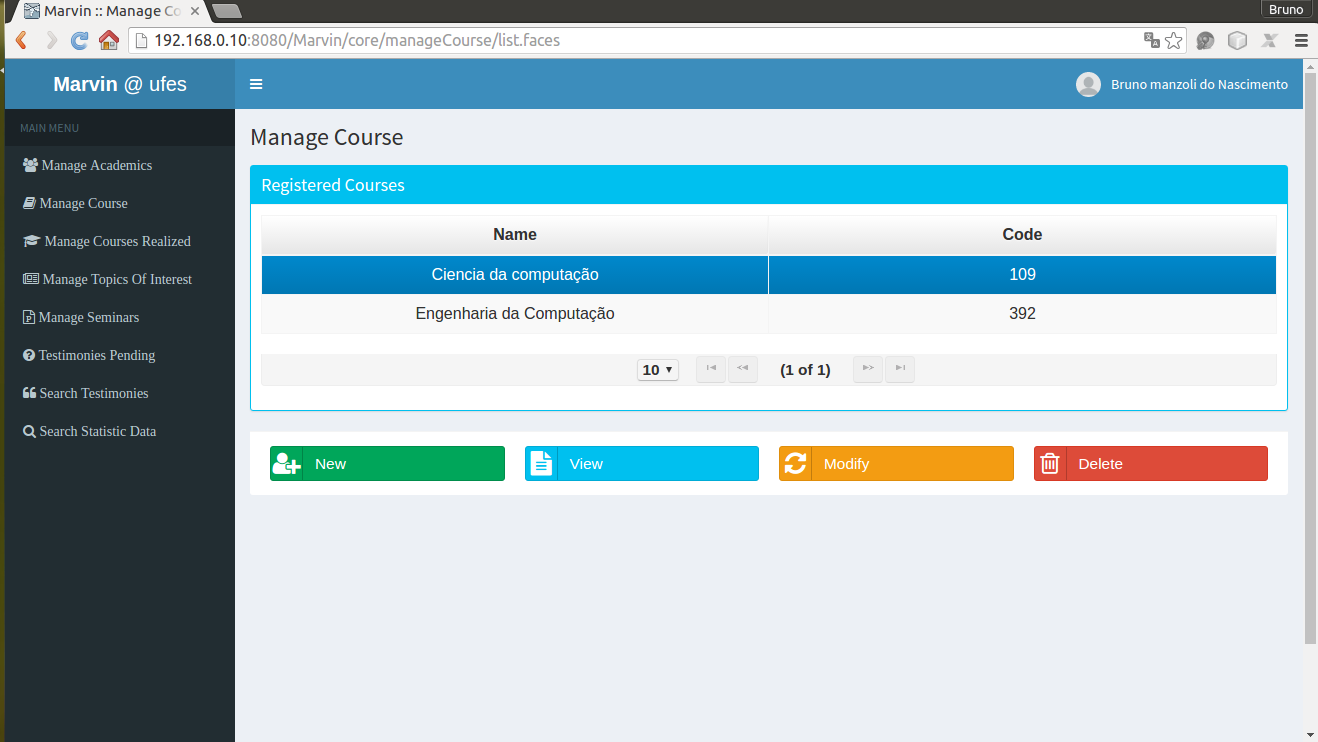
\includegraphics[width=0.75\textwidth]{figuras/projeto/fig-projeto-apresentacao-course-list}
	\caption{SAE - Lista de Curso.}
	\label{fig-projeto-apresentacao-course-list}
\end{figure}


Quando o usuário clicar nos botões \textbf{New} (novo) ou \textbf{View} (visualizar) ou \textbf{Modify} (alterar), sera redirecionado para a pagina de cadastro de um item conforme a Figura~\ref{fig-projeto-apresentacao-course-form}.

\begin{figure}[h]
	\centering
	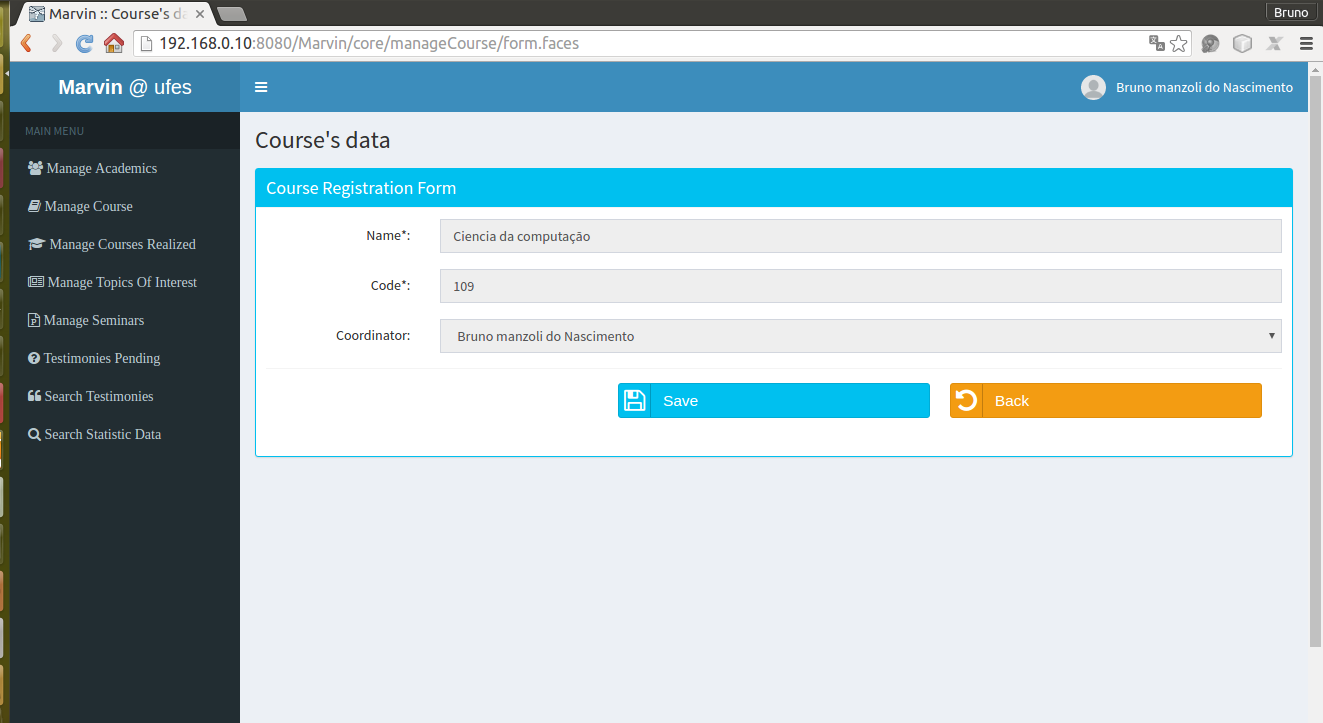
\includegraphics[width=0.75\textwidth]{figuras/projeto/fig-projeto-apresentacao-course-form}
	\caption{SAE - Tela cadastro de Curso.}
	\label{fig-projeto-apresentacao-course-form}
\end{figure}


\newpage
Para exclusão de um item, após clicar no botão ``delete'' será exibido um novo painel para confirmação da exclusão como podemos ver na Figura~\ref{fig-projeto-apresentacao-course-excluir}, na parte inferior da tela informando o item que será excluída e os botões de confirmar a exclusão e de cancelar a exclusão. 

\begin{figure}[h]
	\centering
	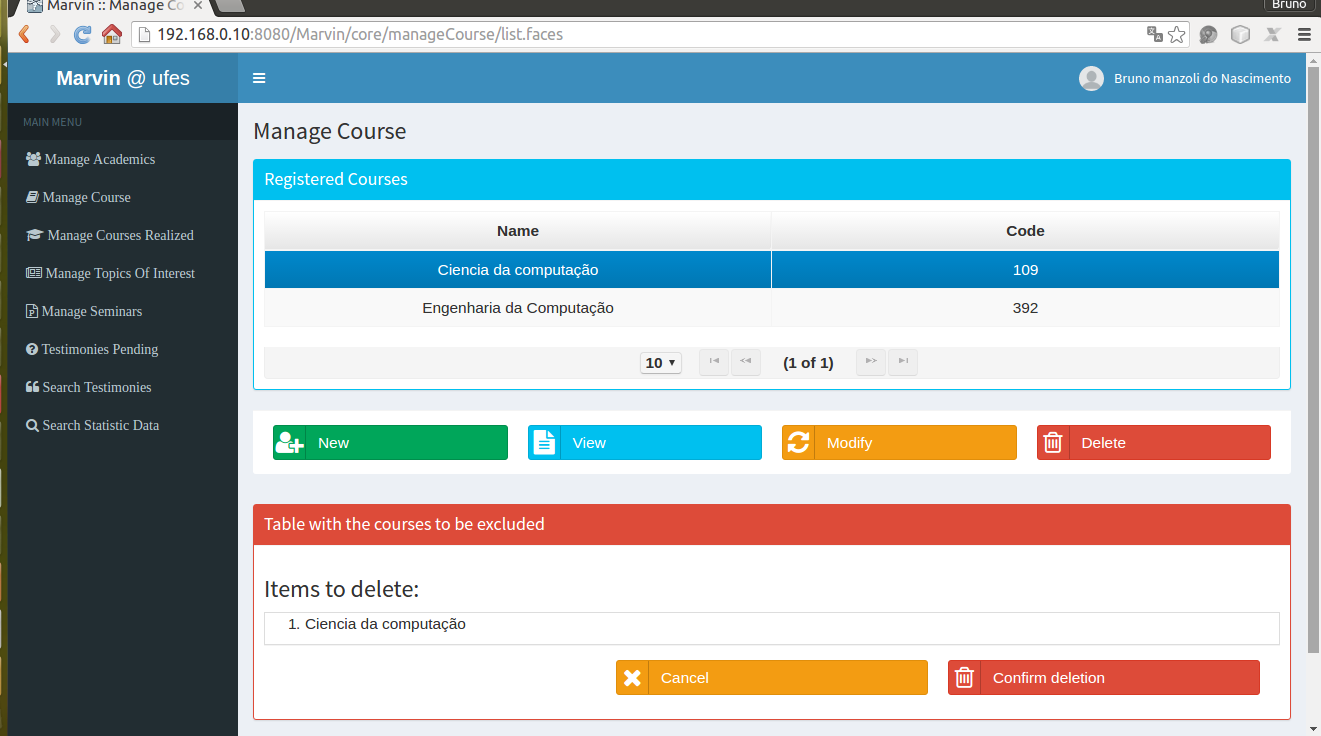
\includegraphics[width=0.75\textwidth]{figuras/projeto/fig-projeto-apresentacao-course-excluir}
	\caption{SAE - Tela exclusão de Curso.}
	\label{fig-projeto-apresentacao-course-excluir}
\end{figure}



A Figura~\ref{fig-projeto-apresentacao-resposiva-buttons} apresenta a telas de listagem de itens e de dados de um item para quem  está utilizando um dispositivo móvel, podemos notar algumas diferenças em relação a visualização para \textit{desktop} como o menu que não aparece e principalmente a disposição dos botões onde eles passam de uma formação horizontal na versão \textit{desktop} para uma vertical na versão \textit{mobile}. Para facilitar e orientar o usuário foram utilizados cores para identificar as funções dos botões como, por exemplo, o botão de criar um novo item tem a cor verde, o de visualizar os dados de um item tem a cor azul.


\begin{figure}[h]
	\centering
	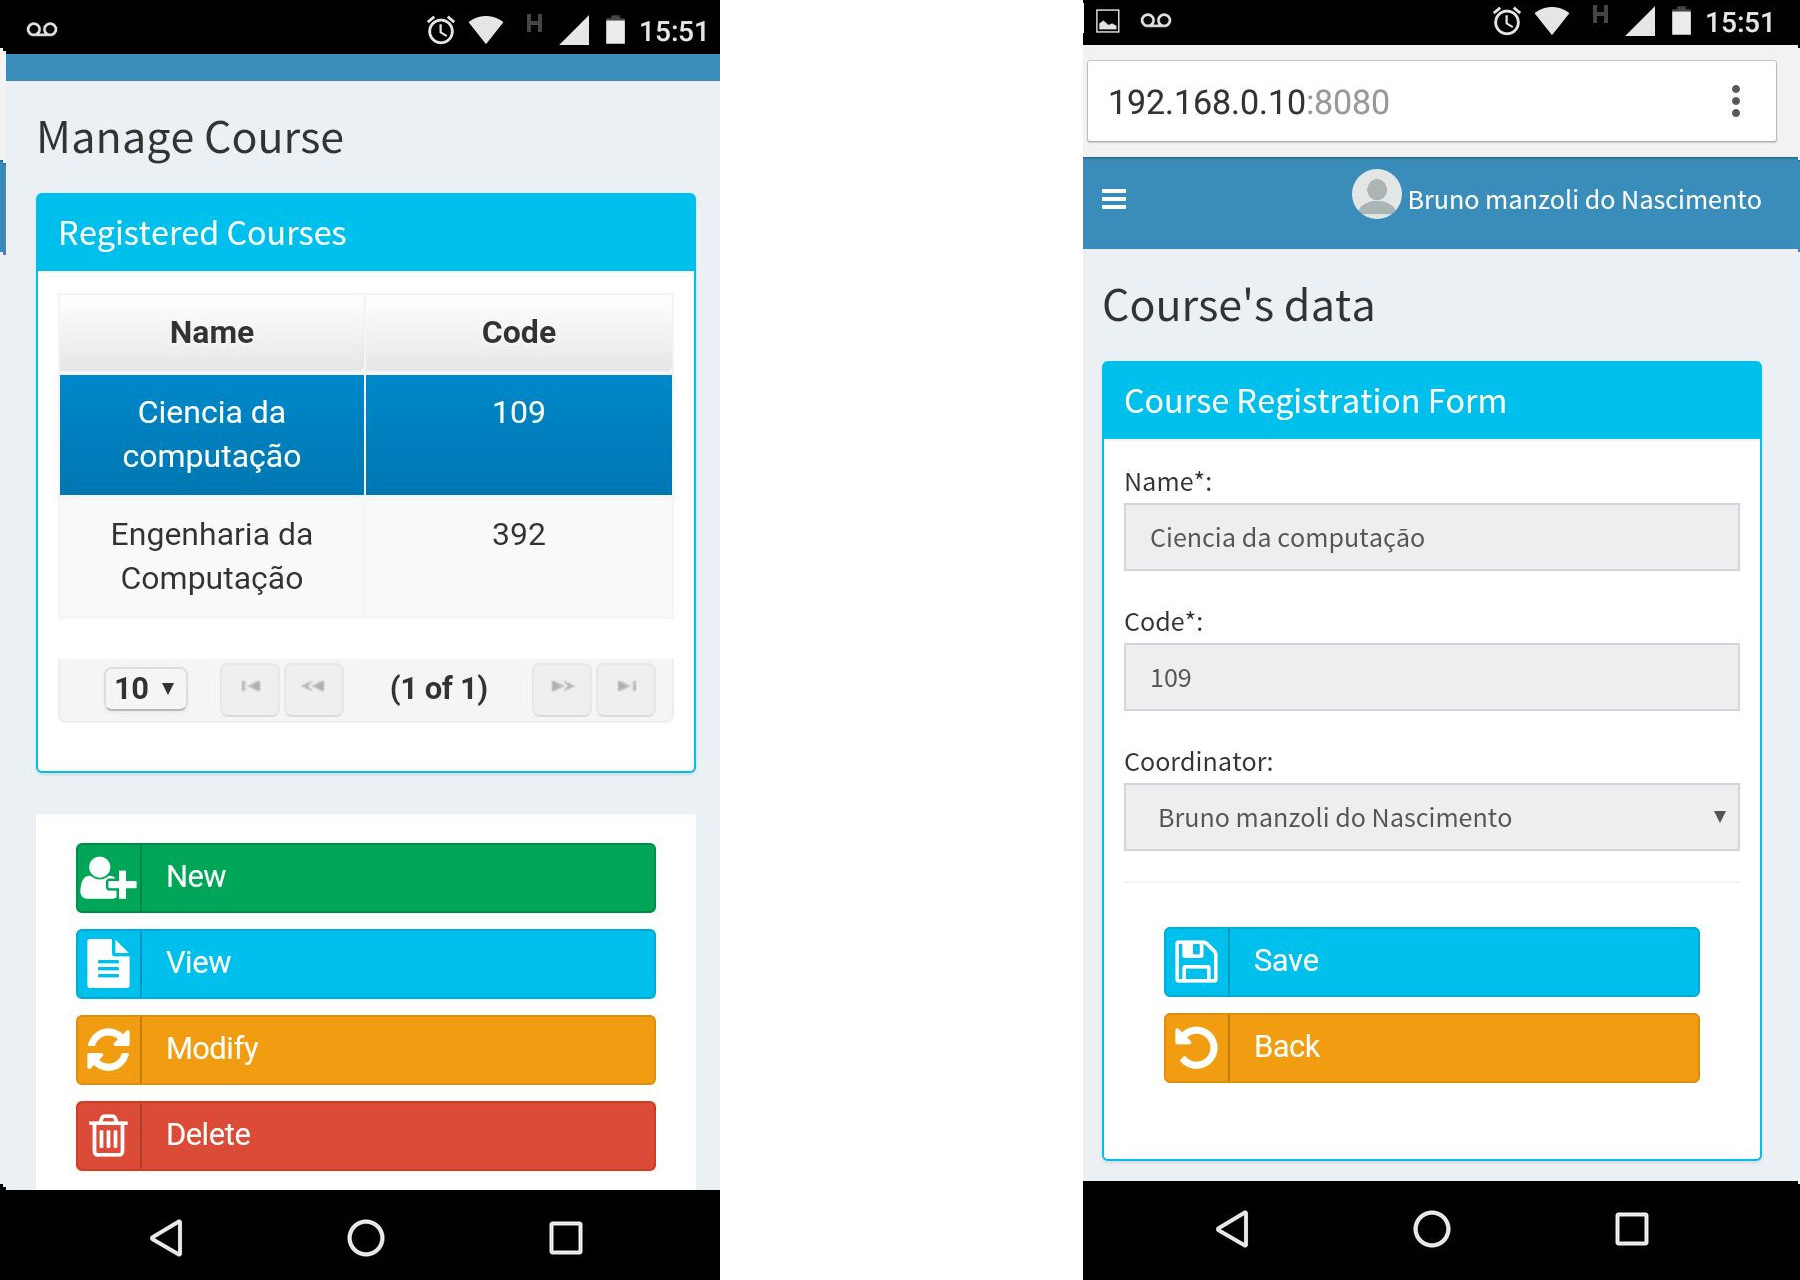
\includegraphics[width=0.75\textwidth]{figuras/projeto/fig-projeto-apresentacao-resposiva-buttons}
	\caption{SAE - Telas mobile.}
	\label{fig-projeto-apresentacao-resposiva-buttons}
\end{figure}


\newpage
As figuras~\ref{fig-projeto-apresentacao-grafico} e~\ref{fig-projeto-apresentacao-tela-grafico-salario} mostram as telas relacionadas ao caso de uso consultar dados estatísticos, onde se tem a tela com as opções de gráficos como por exemplo o de nível salarial, área de atuação, área de formação, entre outros. As figuras também mostram as telas com os gráficos em forma de pizza com as porcentagem que representa cada item da sua legenda.

\begin{figure}[h]
	\centering
	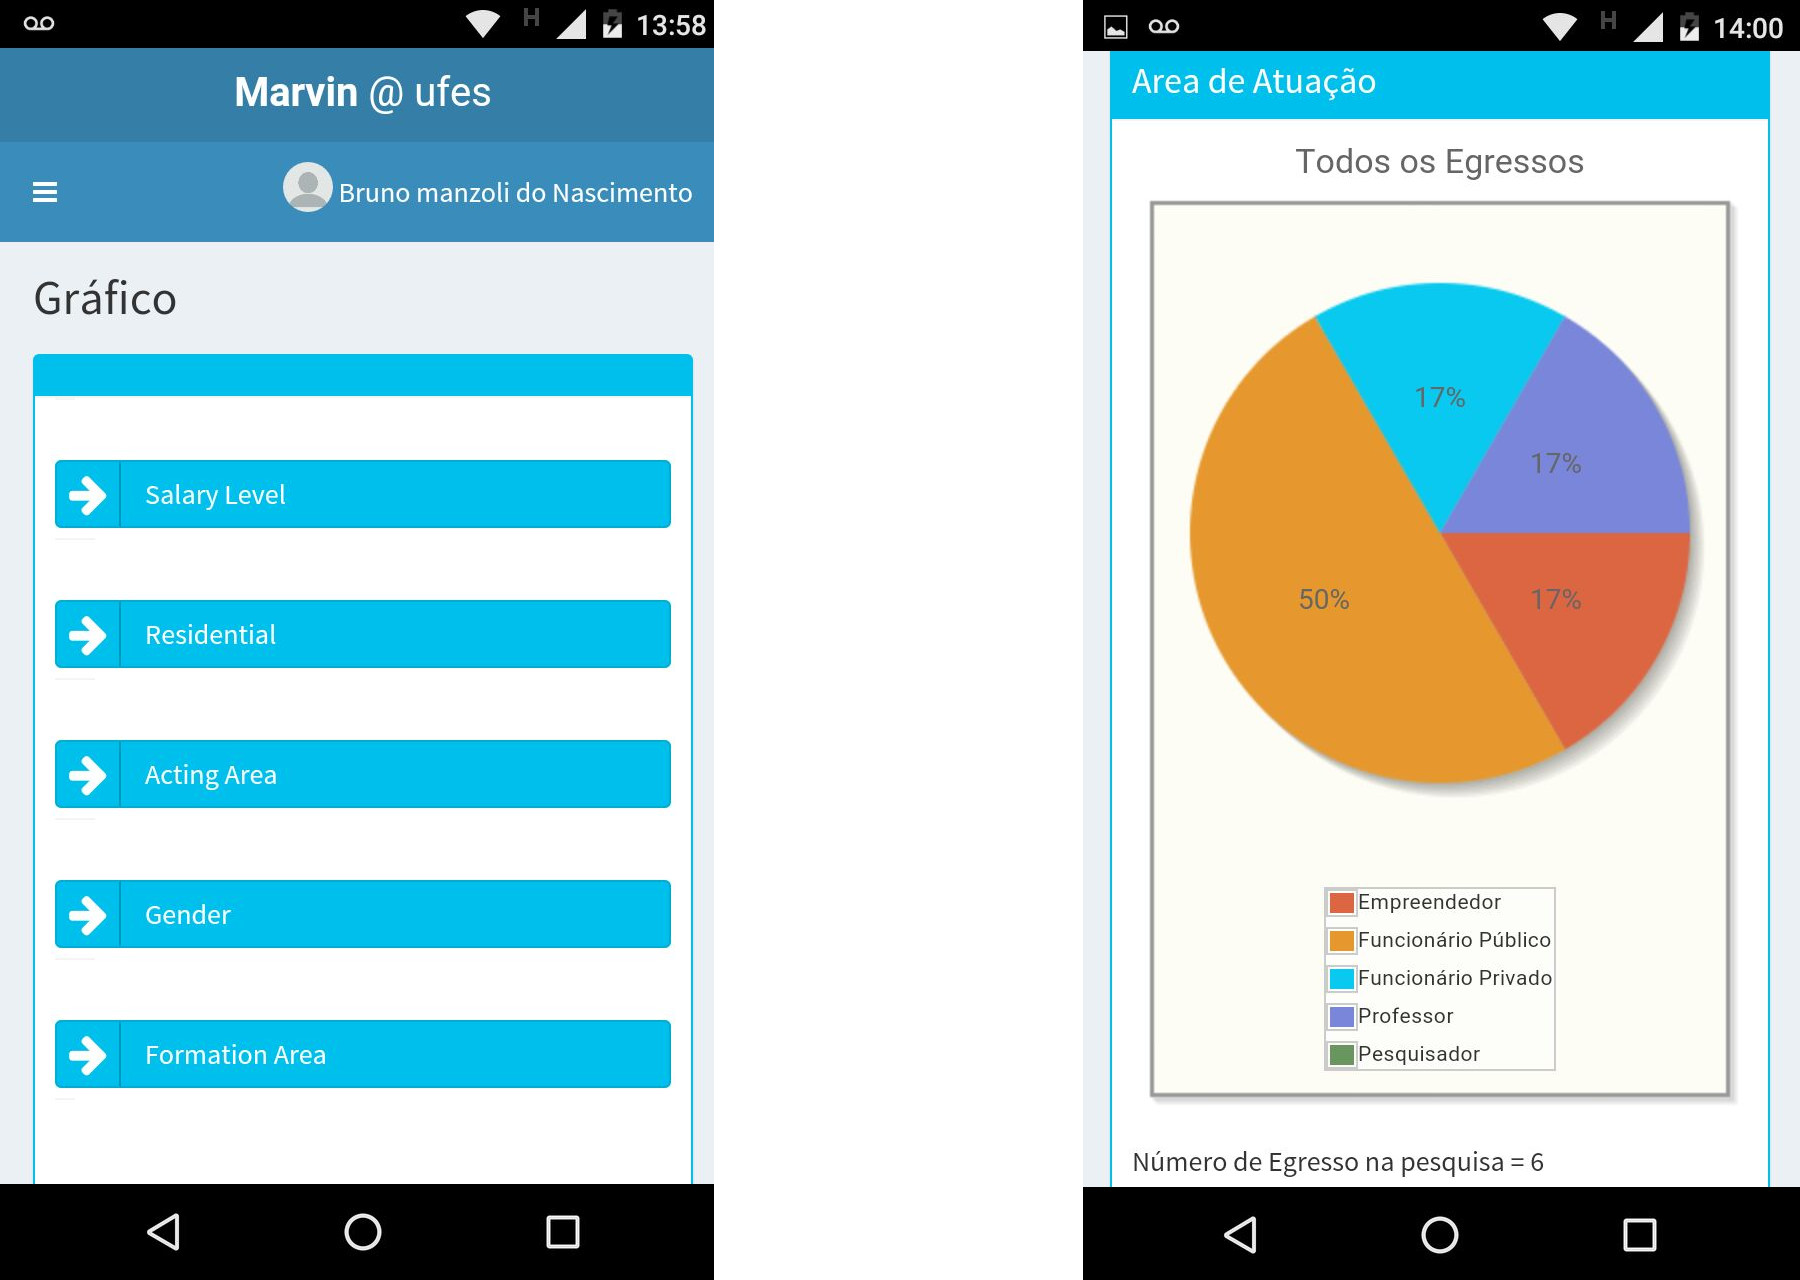
\includegraphics[width=0.75\textwidth]{figuras/projeto/fig-projeto-apresentacao-grafico}
	\caption{SAE - Telas mobile Gráfico.}
	\label{fig-projeto-apresentacao-grafico}
\end{figure}


\begin{figure}[h]
	\centering
	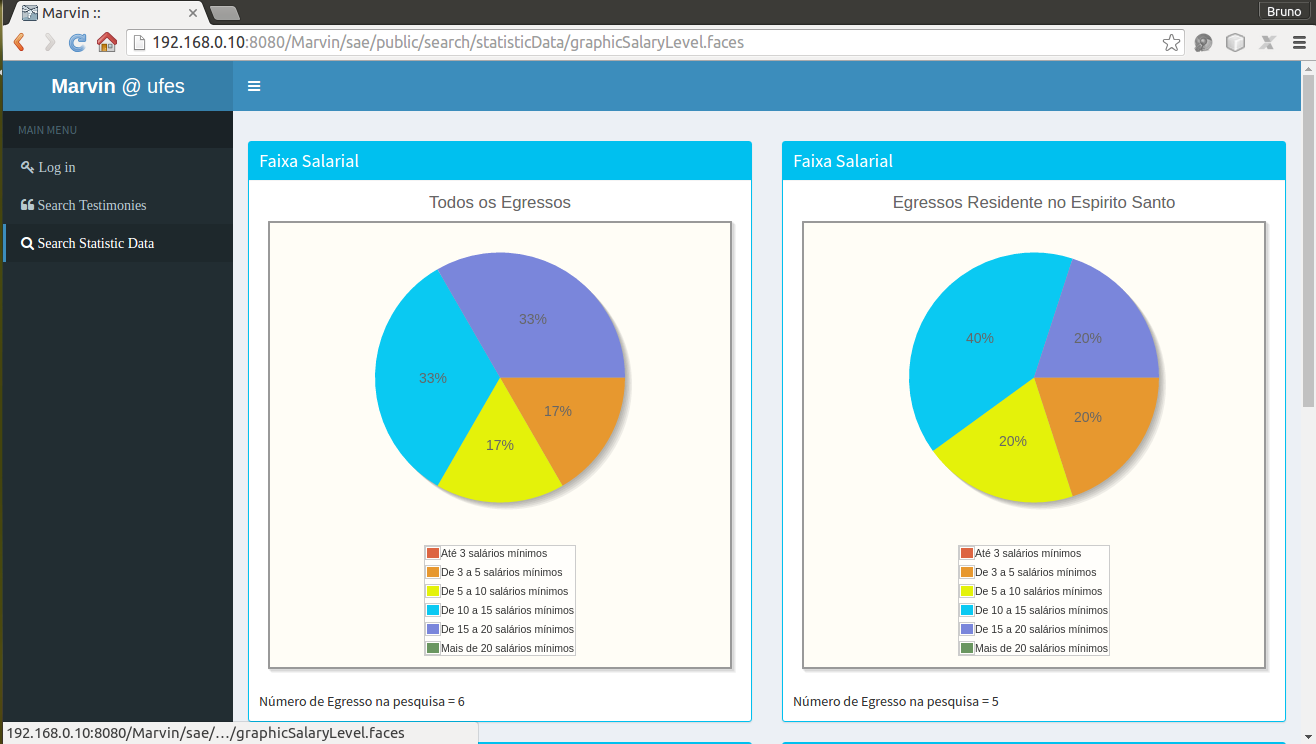
\includegraphics[width=0.8\textwidth]{figuras/projeto/fig-projeto-apresentacao-tela-grafico-salario}
	\caption{SAE - Tela Consulta Faixa Salarial.}
	\label{fig-projeto-apresentacao-tela-grafico-salario}
\end{figure}


\newpage
Para se ter um depoimento divulgado no site antes ele tem que passar por uma avaliação de um administrador, a Figura~\ref{fig-projeto-apresentacao-depoimento-analisar} mostra os depoimento que estão esperando por uma avalização, para avaliar o administrador seleciona o depoimento e clica no botão \textbf{View} (visualizar).
\begin{figure}[h]
	\centering
	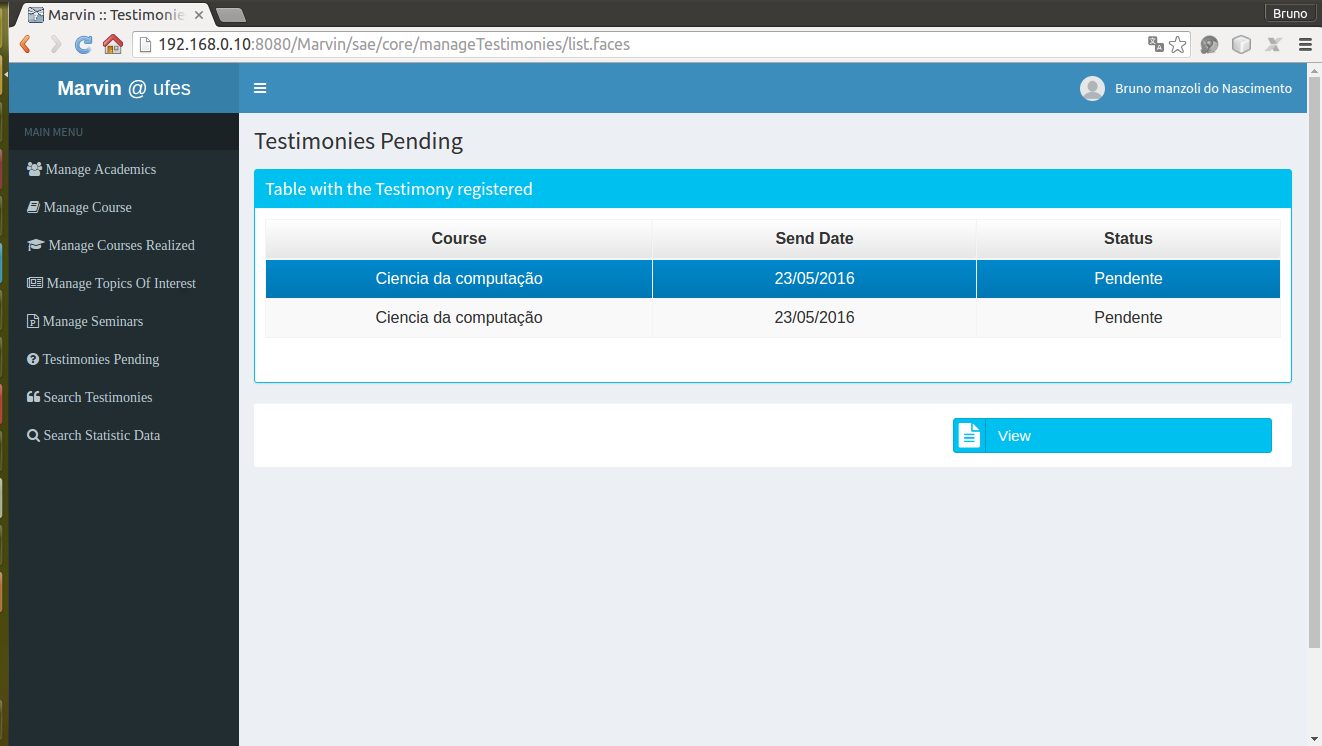
\includegraphics[width=0.8\textwidth]{figuras/projeto/fig-projeto-apresentacao-depoimento-analisar}
	\caption{SAE - Tela Depoimentos á serem analisados.}
	\label{fig-projeto-apresentacao-depoimento-analisar}
\end{figure}

Depois de clicar no botão \textit{view} o administrador será redirecionado para a pagina de avaliação do depoimento como mostra a Figura~\ref{fig-projeto-apresentacao-analise-depoimento}, onde se tem os dados do depoimento no modo de leitura apenas. Assim, o administrador vai apenas clicar no botão \textbf{Approve} (aprovar) ou no botão \textbf{Disapprove} (desaprovar) para aprovar ou desaprovar o depoimento respectivamente.

\begin{figure}[h]
	\centering
	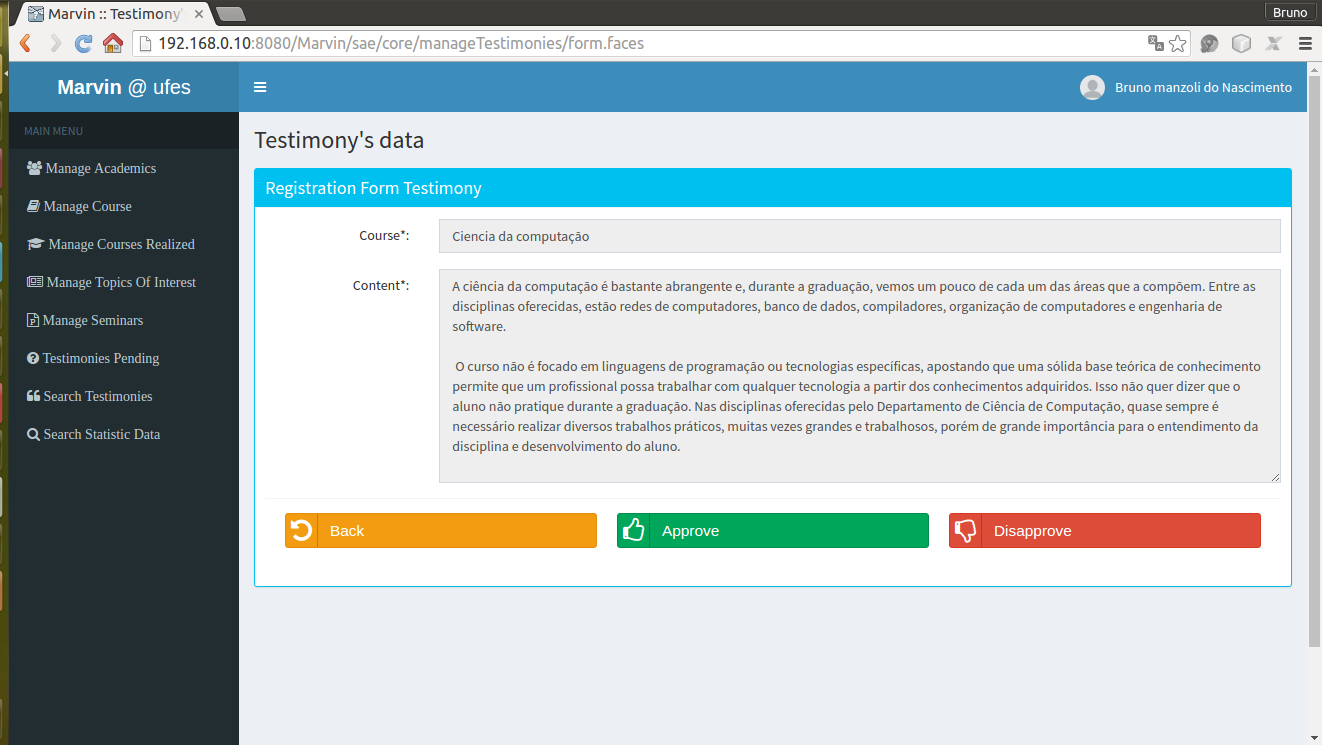
\includegraphics[width=0.8\textwidth]{figuras/projeto/fig-projeto-apresentacao-analise-depoimento}
	\caption{SAE - Tela Análise de Depoimentos.}
	\label{fig-projeto-apresentacao-analise-depoimento}
\end{figure}


\newpage
A Figura~\ref{fig-projeto-apresentacao-tela-depoimentos} mostra como serão divulgados os depoimentos aprovados pelos administradores. Podemos observar nesta figura que são mostrados o nome do egresso, o seu depoimento e a data que ele o enviou. Para os casos onde o egresso não queira se identificado como o autor do depoimento, no lugar do nome aparecerá que o depoimento é anônimo.


\begin{figure}[h]
	\centering
	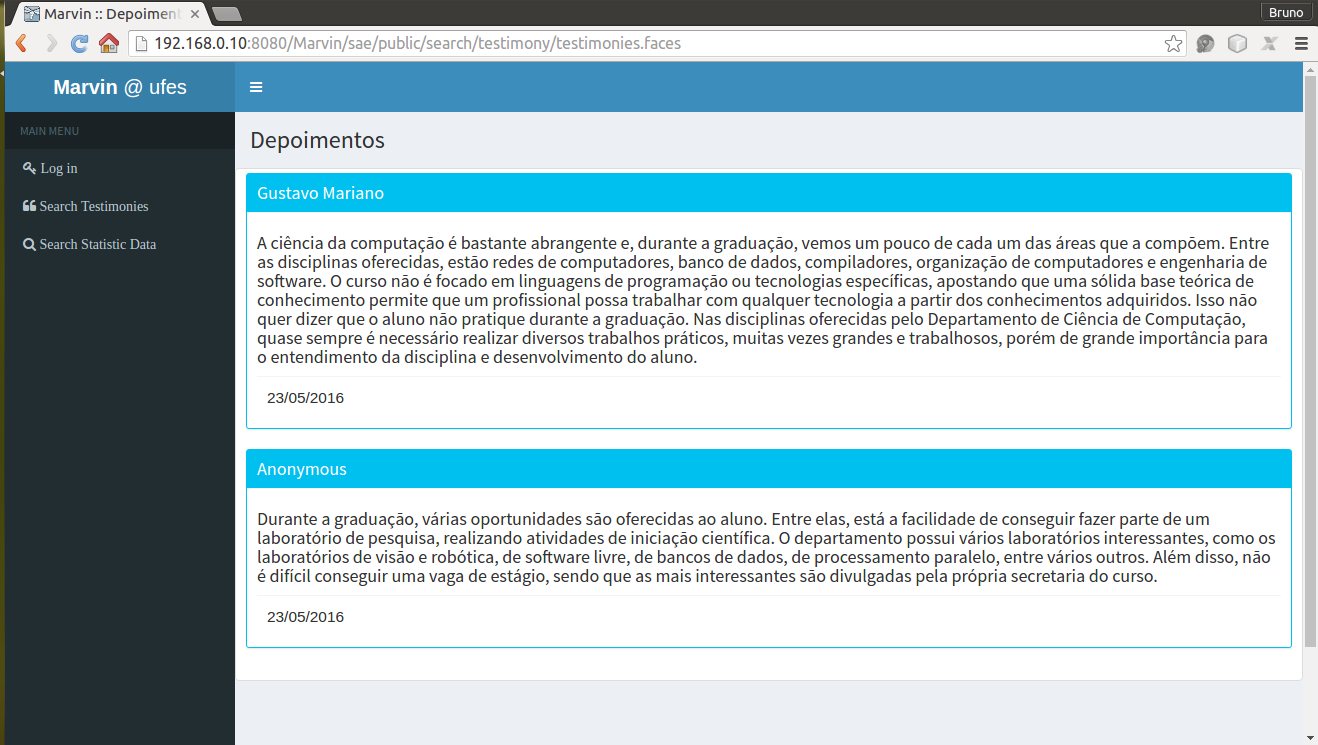
\includegraphics[width=0.8\textwidth]{figuras/projeto/fig-projeto-apresentacao-tela-depoimentos}
	\caption{SAE - Tela Consulta Depoimentos.}
	\label{fig-projeto-apresentacao-tela-depoimentos}
\end{figure}














